\chapter{Validación de la herramienta numérica }
\graphicspath{{figs/cap4/}}
\label{cap4}

En el presente capítulo se realiza la descripción de los problemas con transferencia de calor para fluidos multifásicos con cambio de fase llevados a cabo para validar los códigos numéricos desarrollados, siendo éstos la \textit{Construcción de Maxwell}, la \textit{Estratificación de un fluido Van der Waals con temperatura no uniforme} y la \textit{Generación de burbujas en una superficie horizontal calefaccionada}.

\section{Construcción de Maxwell}

En esta sección se explica el procedimiento por el que a partir de una EOS, se puede obtener las densidades de coexistencia de un fluido para un dado valor de presión y temperatura. Dicho procedimiento se llama Construcción de Maxwell, donde necesariamente la EOS con la que se modela el fluido debe permitir la coexistencia de densidades para sus variables de estado. Para la resolución de éste problema solo se utiliza la ecuación hidrodinámica del LBM.

En el desarrollo del Cap. (\ref{cap2}) se adoptó como EOS del presente trabajo, la ecuación de VdW Ec. (\ref{eq:p_eos_4}) que describe el comportamiento de un gas real y permite la coexistencia de diferentes densidades para igual presión y temperatura:
\begin{align}
	p = \frac{R T}{V_m - B} - A {\left(\frac{1}{V_m}\right)}^2
	\label{eq:p_eos_4}
\end{align}

La Ec. (\ref{eq:p_eos_4}) puede ser representada gráficamente en un diagrama $P - V_m$. A modo de ejemplo se presenta el diagrama para el caso del dióxido de carbono ($CO_2$) a tres temperaturas distintas ver Figura (\ref{fig:P_V_CO2}).  La temperatura de interés es la de $T = 270 \> K$, donde se vislumbra que en $p = 44,08 \> atm$ la gráfica se intersecta en tres valores de $V_m$, siendo dos de ellos estables; por lo que se observa que hay dos volúmenes molares de coexistencia, indicando las fases líquido y gaseosa \cite{huang2015multiphase}. Además se forman las áreas \textbf{A1} y \textbf{A2} delimitadas por la curva $P - V_m$ y la línea de presión constante a $p = 44,08 \> atm$. 

\begin{figure}[htbp]
	\centering
	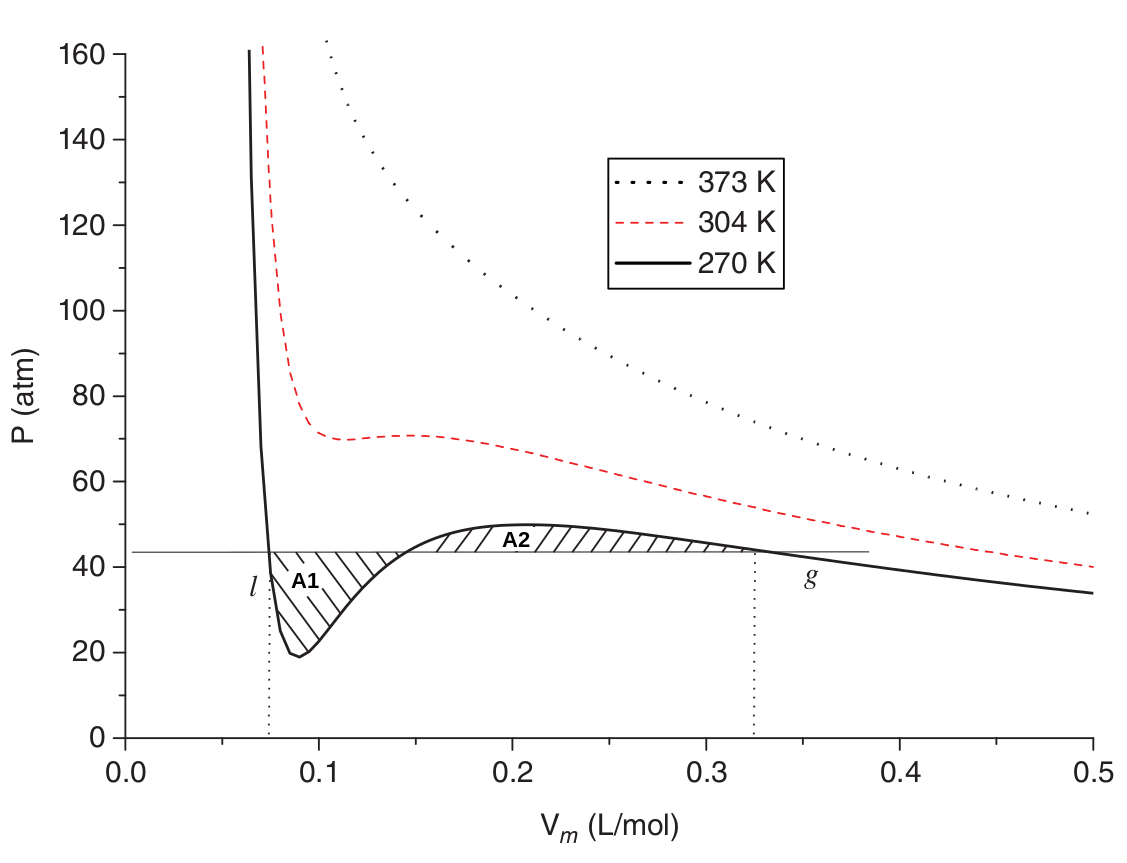
\includegraphics[width=.8\textwidth]{figs/cap4/Diagrama_P_V_del_CO2_Multiphase_LBM}
	\caption{Diagrama $P - V_m$ de la EOS de VdW del $CO_2$ con las constantes $A = 3,592$ y $B = 0,04267$, representando para $T = 270 \> K$ los volúmenes molares del líquido y gas. \textbf{A1} y \textbf{A2} son el área encerrada entre la curva $P - V_m$ a $T = 270 \> K$ y la línea de presión constante a  $p = 44,08 \> atm$ \cite{huang2015multiphase}.}
	\label{fig:P_V_CO2}	
\end{figure}

La construcción de Maxwell, también llamada regla de igualdad de áreas, indicada en la Ec. (\ref{eq:maxwell_Construction}), es un procedimiento analítico para encontrar las densidades de coexistencia del líquido y gas. Al realizar la integral propuesta surge que las áreas \textbf{A1} y \textbf{A2} de la Figura (\ref{fig:P_V_CO2}) deben ser iguales.

\begin{equation}
\int_{V_{m,l}}^{V_{m,g}} P \> d V_m = p_0 (V_{m,l} -  V_{m,g})
\label{eq:maxwell_Construction}
\end{equation}

En donde $P$ es la presión de la EOS y $p_0$ es una presión constante.

La Ec. (\ref{eq:p_eos_4}) puede reescribirse como:

\begin{equation}
	p_{EOS} = \frac{\rho R T}{1- \rho b} - a {\rho}^{2} 
	\label{eq:p_VdW_rho}
\end{equation}

donde $\rho = \frac{1}{v}$, siendo $v = \frac{V_m}{M}$ el volumen másico. De esta forma reescribiendo la integral de la Ec. (\ref{eq:maxwell_Construction}) usando la presión de Ec. (\ref{eq:p_VdW_rho}), pueden obtenerse los valores de coexistencia $\rho_l$ y $\rho_g$ para las fases líquida y gaseosa, respectivamente. 

La coexistencia de fases tiene lugar a temperaturas inferiores a una temperatura crítica ($T_c$). En el ejemplo mostrado de la Figura (\ref{fig:P_V_CO2}) $T_c = 304 \> K$. Analíticamente $T_c$ surge de aplicar el criterio de la primera y segunda derivada a la Ec.(\ref{eq:rho}) como se indica en Ec.(\ref{eq:criterio_1_2_deriv}) y se deben conocer los parámetros \textit{a} y \textit{b}.

\begin{equation}
	\frac{\partial\> p}{\partial\> V_{m}} = 0 \qquad \qquad \frac{\partial^{2} \> p}{\partial\> {V_{m}}^{2}} = 0
	\label{eq:criterio_1_2_deriv}
\end{equation}

Realizando adecuadamente la adimensionalización  de la Ec.(\ref{eq:p_VdW_rho}) se puede graficar una curva de coexistencia $T_r - \rho_r$, donde $T_r = \frac{T}{T_c}$, $\rho_r = \frac{\rho}{\rho_c}$ y $T_c$ es calculado a partir de los parámetros \textit{a} y \textit{b} asignados al fluido de estudio. Es de importancia destacar que las curvas de coexistencia dependen de la EOS que se esté utilizando para describir el comportamiento del fluido. En el caso de estudio analizado, la EOS es de VdW y la curva de coexistencia es universal, independientemente de los parámetros \textit{a} y \textit{b}, debido a que se encuentra normalizada por unidades críticas.

Para un fluido con una EOS de VdW con sus respectivos parámetros \textit{a} y \textit{b}, se puede calcular los valores de $T_c$ y $\rho_c$. Se inicializa aleatoriamente la densidad del fluido mencionado alrededor de $\rho_c$, en una cavidad bidimensional que se encuentra a una dada temperatura. A consecuencia de la evolución temporal se producirá la separación de las fases del mismo, produciéndose una coexistencia de fases. Por medio de la obtención de las densidades de coexistencia para distintas temperaturas iniciales, se puede reconstruir la curva de coexistencia analítica. De esta forma, el problema de construcción de Maxwell puede emplearse para validar la implementación de las ecuaciones LBM hidrodinámicas.

En este problema, se valida la curva de coexistencia $T_r - \rho_r$ calculada analíticamente para un fluido con una EOS de VdW, como la observada en la Figura (\ref{fig:v_760_MxC_c_simple}). 

\subsection{Validación}

La validación de este problema se hizo utilizando los parámetros $a =0,5$ y $b = 4,0$; para un tamaño de malla de 201 x 201 nodos y $T_r$ variando con un paso de $0,025$ en el rango de $[0,6 - 0,975]$.  El valor de los parámetros utilizados de LBM son los siguientes:

\begin{align*}
diag(\mathbf{\Lambda}) = 
\begin{bmatrix}
1.0 & 0.8 & 1.1 & 1.0 & 1.1 & 1.0 & 1.1 & 0.8 & 0.8 \\
\end{bmatrix}\\
G = -1.0 \quad c = 1.0 \quad \sigma = 0.125 \quad a = 0.5 \quad b = 4.0 \\
\mathbf{g} = (0.0 \quad 0.0 \quad 0.0 ) \qquad \rho_c = \frac{1}{12} \qquad T_c = 0.037037037
\end{align*}

La Figura(\ref{fig:v_760_MxC_c_simple}) muestra la validación del código realizado en \textsc{C} para simple precisión en una CPU Intel Core i7-3770; con distintos parámetros $\sigma$ del modelo MRT, donde se observa que el valor de $\sigma = 0,125$ es el que mejor ajusta a la curva de coexistencia como se discute en \cite{fogliatto2018modelado}. Por otro lado, en la Figura (\ref{fig:v_760_MxC_cuda_simple}) se muestran los resultados obtenidos con el código realizado en \textsc{Cuda C}, y ejecutado en la GPU correspondiente

Los resultados, que se muestran en las Figuras (\ref{fig:v_760_MxC_c_simple}) y (\ref{fig:v_760_MxC_cuda_simple}), se realizaron en 50000 pasos de tiempo en cada uno de los valores de $T_r$. Puede observarse que los valores obtenidos de las densidades de coexistencia de fases entre los códigos de \textsc{C} y \textsc{Cuda C} resultan similares.

Al comparar los resultados luego de la validación de las densidades de fase entre \textsc{C} y \textsc{Cuda C} para doble precisión, se obtuvo que poseen el mismo valor numérico. 

\begin{figure}[h!]
	\centering
	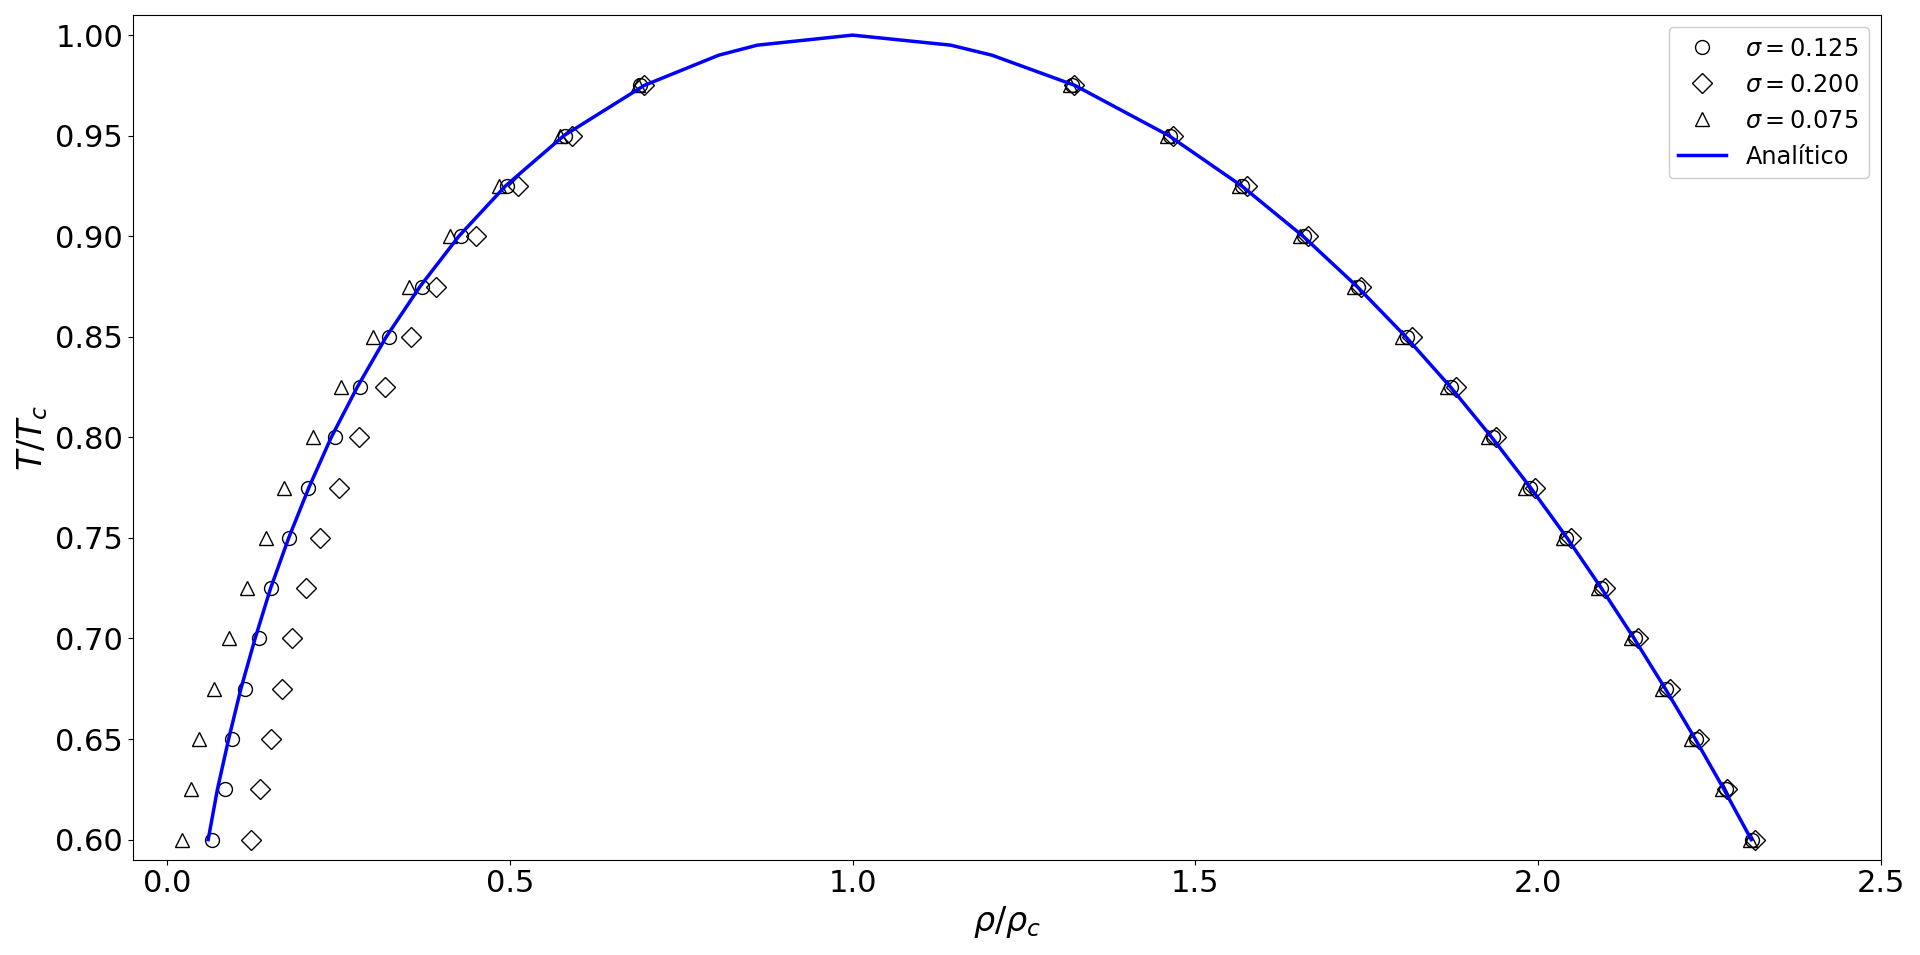
\includegraphics[width=\textwidth]{figs/cap4/v_760_MxC_c_simple}
	\caption{Curva de coexistencia de fases para un fluido de VdW con los parámetros $a = 0,5 $ y $b = 4,0 $, obtenida en simple precisión en la CPU Intel Core i7-3770 en el código desarrollado en \textsc{C}. Los puntos corresponden a valores del parámetro libre del modelo MRT de $\sigma = 0.075[\bigtriangleup]$	 $\sigma = 0.125[\bigcirc]$ y $\sigma = 0.200[\diamondsuit]$ }
 	\label{fig:v_760_MxC_c_simple}	
\end{figure}

\begin{figure}[h!]
	\centering
	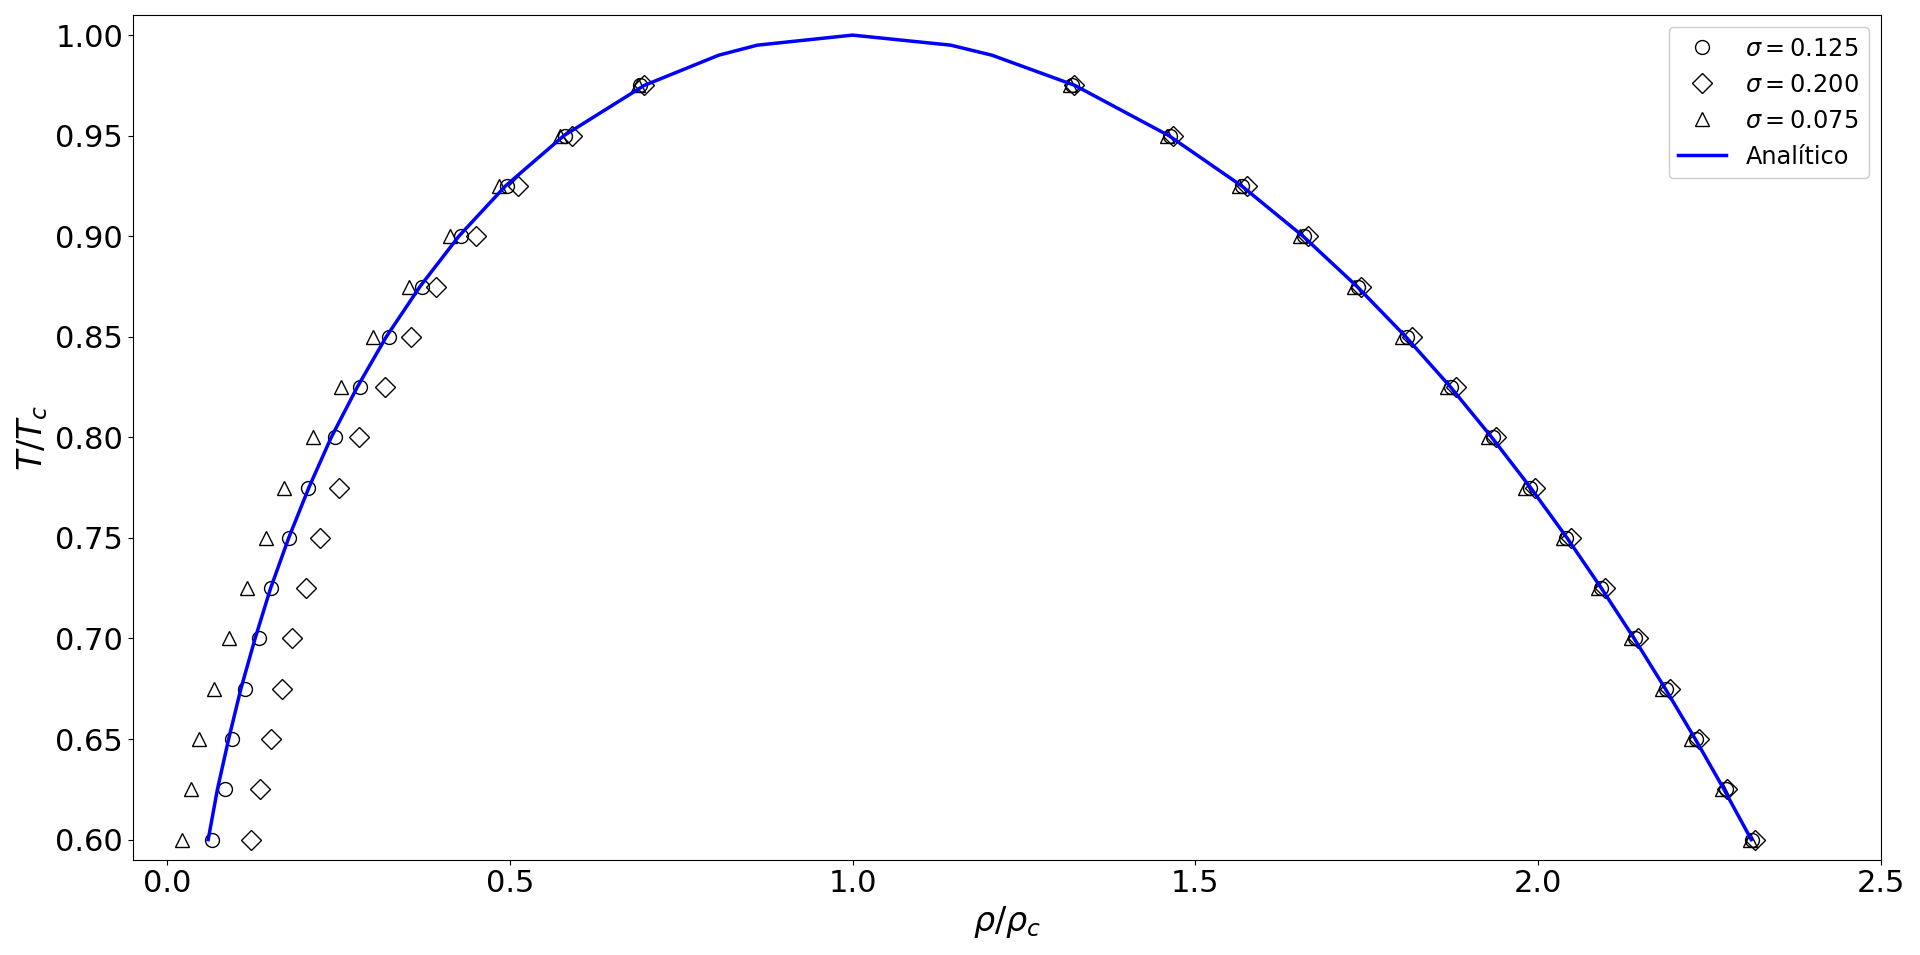
\includegraphics[width=\textwidth]{figs/cap4/v_760_MxC_cuda_simple}
	\caption{Curva de coexistencia de fases para un fluido de VdW con los parámetros $a = 0,5 $ y $b = 4,0 $, obtenida en simple precisión en la GPU NVIDIA GeForce GTX 760 en el código desarrollado en \textsc{Cuda C}. Los puntos corresponden a valores del parámetro libre del modelo MRT de $\sigma = 0.075[\bigtriangleup]$	 $\sigma = 0.125[\bigcirc]$ y $\sigma = 0.200[\diamondsuit]$ }
	\label{fig:v_760_MxC_cuda_simple}	
\end{figure}



\newpage
\subsection{Comparación de precisiones}

La Figura (\ref{fig:v_760_MxC_c_comparacion}) muestra los resultados de las densidades de coexistencia de fases para simple y doble precisión, no siendo apreciable la diferencia.

\begin{figure}[htbp]
	\centering
	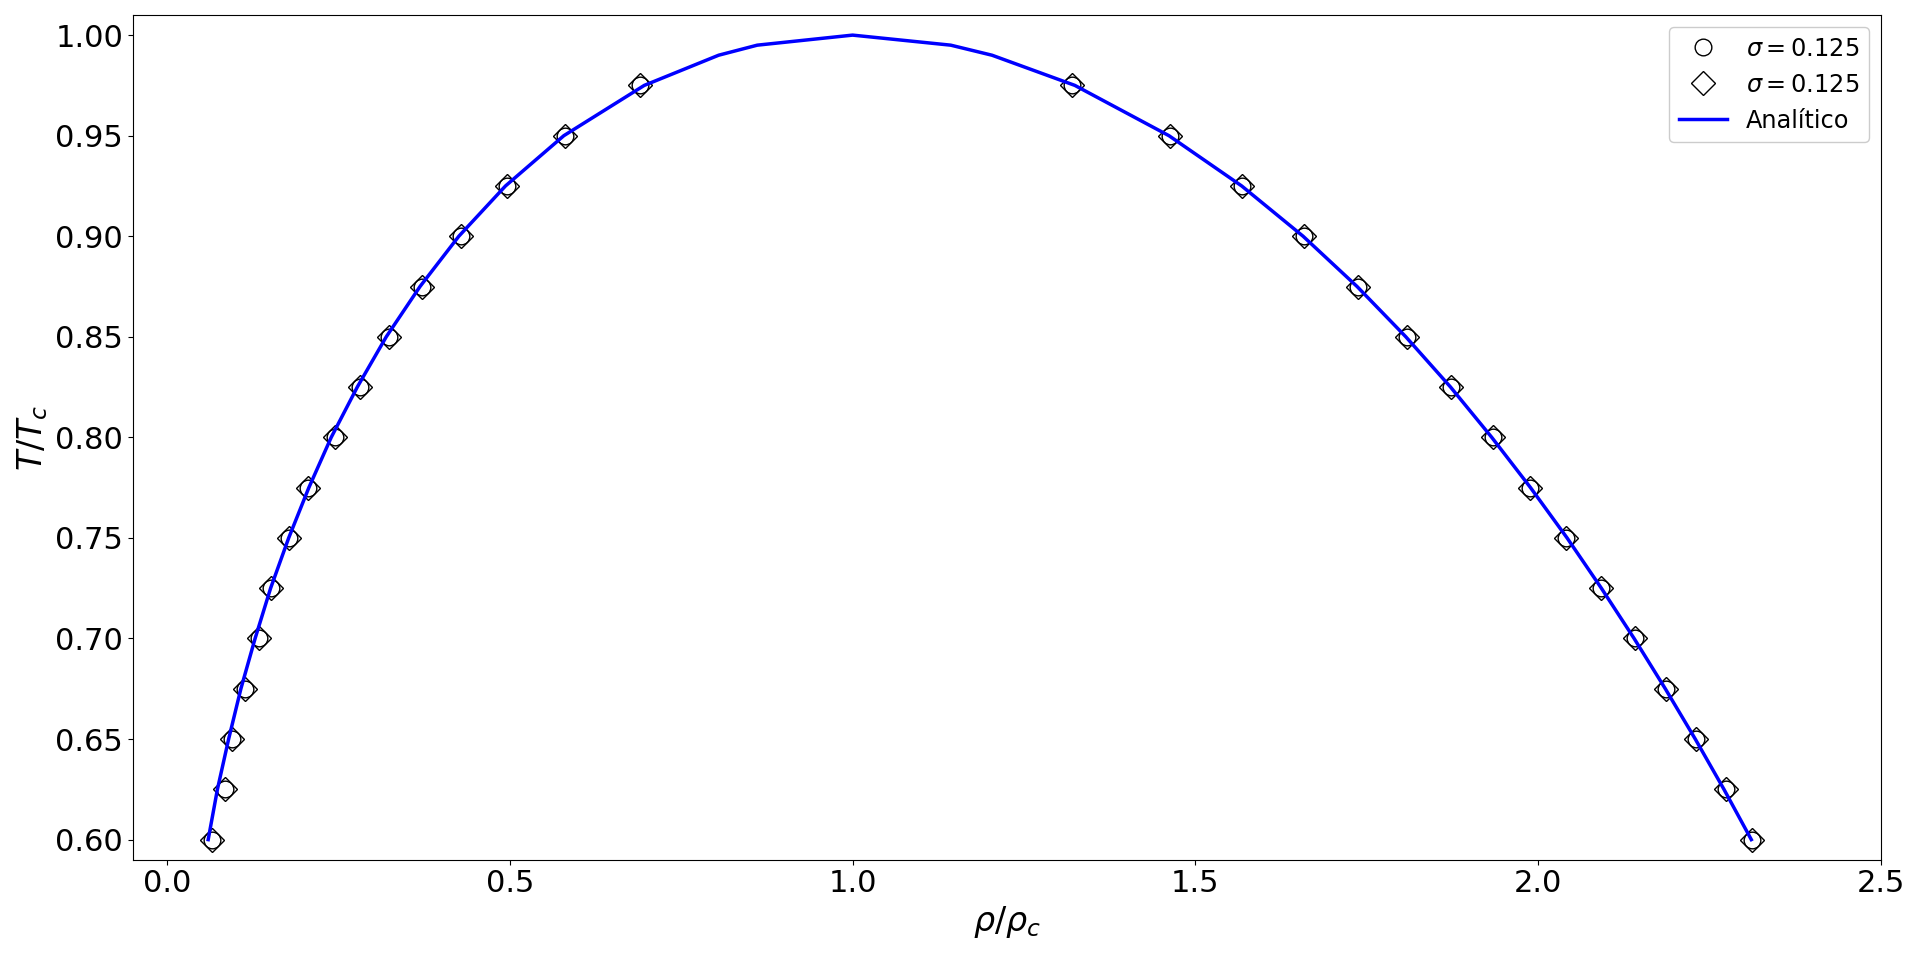
\includegraphics[width=\textwidth]{figs/cap4/v_760_MxC_c_comparacion}
	\caption{Curva de coexistencia de fases para un fluido de VdW con los parámetros: $a = 0,5 $ y $b = 4,0 $. Los puntos corresponden a los valores obtenidos en simple precisión [$\bigcirc$] y doble precisión [$\diamondsuit$] en la GPU NVIDIA GeForce GTX 760 en el código desarrollado en \textsc{C}.} 
	\label{fig:v_760_MxC_c_comparacion}	
\end{figure}


%La Tabla (\ref{tab:comp_MxC_precisiones_10}) contiene los valores de las densidades de coexistencia: analítico, y los obtenidos mediante el código en simple precisión y doble precisión. De la Figura (\ref{fig:v_760_MxC_c_comparacion}) se observa que se ajusta mejor al resultado analítico la fase líquida que la fase gaseosa, por ello la Tabla (\ref{tab:comp_MxC_precisiones_10}) presenta esta diferenciación.

El error en la aproximación a la solución analítica se mide como la distancia entre los vectores de densidad de fase obtenido y el analítico. La distancia se calculó por medio de la Norma Euclídea, siendo calculada la distancia entre dos vectores \textbf{\textit{A}} y \textbf{\textit{B}} con \textit{i} elementos como indica la Ec.(\ref{eq:norma_euclidea}):

\begin{align}
dist(\mathbf{A},\mathbf{B}) = \sqrt{\sum_i {\left( a_i - b_i \right)}^2  }
\label{eq:norma_euclidea}
\end{align}

%A partir de los resultados obtenidos, que muestra la Tabla (\ref{tab:comp_MxC_precisiones_10}) en cuanto a la distancia de los vectores se observa que en doble precisión los resultados se aproximan mejor en la densidad de coexistencia de la fases, en la fase gaseosa; mientras que para la densidad de coexistencia de fase, de la fase líquida, se aproxima mejor mediante simple precisión. 

La mayor diferencia porcentual hallada para la distancia en la fase gaseosa, es que en simple precisión es 0,0034 \% mayor que en doble precisión. Para la fase líquida se obtuvo que en doble precisión es 0,0491 \% mayor la distancia que en simple precisión.


%% Please add the following required packages to your document preamble:
% \usepackage{multirow}
\begin{table}[h!]
\centering
%\resizebox{17cm}{!}{
	\begin{tabular}{|c|c|c|c|c|c|c|}
	\hline
	& \multicolumn{3}{c|}{${\rho_{r}}_{\>gaseoso}$}      & \multicolumn{3}{c|}{${\rho_{r}}_{\>líquido}$} \\ \hline
	$\mathbf{T_r}$    & \textbf{Analítico}      & \textbf{Simple}       & \textbf{Doble}     & \textbf{Analítico}      & \textbf{Simple}     & \textbf{Doble}   \\ \hline
	0.600 & 0.0599097 & 0.0653772 & 0.0653724 & 1.32424  & 1.31956 & 1.31975 \\ \hline
	0.625 & 0.0733723 & 0.0848112 & 0.0847656 & 1.46149  & 1.46239 & 1.4624  \\ \hline
	0.650 & 0.0897449 & 0.0951336 & 0.095124  & 1.56762  & 1.56858 & 1.56859 \\ \hline
	0.675 & 0.107606  & 0.113153  & 0.113147  & 1.56762  & 1.65819 & 1.65821 \\ \hline
	0.700 & 0.128332  & 0.13353   & 0.133511  & 1.6572   & 1.73703 & 1.73704 \\ \hline
	0.725 & 0.150966  & 0.15182   & 0.151811  & 1.73595  & 1.80812 & 1.80813 \\ \hline
	0.750 & 0.177353  & 0.177323  & 0.177319  & 1.80706  & 1.87326 & 1.87328 \\ \hline
	0.775 & 0.206739  & 0.206086  & 0.206075  & 1.87233  & 1.93364 & 1.93364 \\ \hline
	0.800 & 0.23938   & 0.244229  & 0.244223  & 1.93243  & 1.98754 & 1.98759 \\ \hline
	0.825 & 0.277393  & 0.281299  & 0.281284  & 1.98899  & 2.04083 & 2.04085 \\ \hline
	0.850 & 0.319677  & 0.323471  & 0.323456  & 2.0423   & 2.09124 & 2.09124 \\ \hline
	0.875 & 0.368925  & 0.371915  & 0.371891  & 2.09234  & 2.14114 & 2.14117 \\ \hline
	0.900 & 0.425549  & 0.428416  & 0.428335  & 2.14012  & 2.18665 & 2.18665 \\ \hline
	0.925 & 0.493618  & 0.495973  & 0.495947  & 2.18563  & 2.23017 & 2.23019 \\ \hline
	0.950 & 0.493618  & 0.580402  & 0.580368  & 2.22933  & 2.27407 & 2.27411 \\ \hline
	0.975 & 0.578746  & 0.690126  & 0.690247  & 2.27117  & 2.312   & 2.312   \\ \hline
	\textbf{Distancia} & -         & 2.05233   & 2.05226   & -        & 0.14234 & 0.14241 \\ \hline
\end{tabular}%}
    \caption{Comparación de las precisiones con respecto a cuánto se acercan al valor analitico, tanto para doble, como simple precision, la norma utilizada para medir la distancia de los vectores es la norma  euclídea. Para el problema de la Construcción de Maxwell con la GPU NVIDIA Geforce GTX 760.}
    \label{tab:comp_MxC_precisiones_10}
    \end{table}



\newpage

\subsection{Speed Up}

En la presente sección se muestran las mejoras en el tiempo de cálculo realizados para el código de \textsc{C} y \textsc{Cuda C}. El índice \textit{Speed Up} (SU) calcula la mejora en el tiempo de cálculo entre códigos y se obtiene mediante la Ec.(\ref{eq:speedup}), siendo \textit{t} el tiempo de cálculo y \textit{p} significa comparación entre precisiones. La comparación se realizó en simple y doble precisión para las dos (2) PC detalladas en la Sec. (\ref{sec_pc}).
\begin{align}
	SU = \frac{t_{\>C}}{t_{\>Cuda \> C}} & & 	{SU}_p = \frac{t_{\>doble \> precision}}{t_{\>simple \> precision}} 
	\label{eq:speedup}
\end{align}
Para calcular el \textsc{SU} de éste problema, se tomó una $T_r$ fija y se varió el tamaño de la grilla, de manera que ésta siempre fuese cuadrada, respetando un número de nodos de potencia de 2 en los lados del cuadrado. La cantidad de \textit{thread blocks} que se utilizó para realizar la comparación en el código de \textsc{CUDA} fueron de potencia de 2.

\subsubsection{NVIDIA GeForce GTX 760}

Los tamaños de grilla que se utilizaron para realizar las pruebas de tiempo de esta placa, varían entre 16x16 nodos hasta 2048x2048 nodos. La cantidad de \textit{thread blocks} que se utilizó fueron de 1 a 512.

Las Figuras (\ref{fig:s_760_MxC_simple_1.0}) y (\ref{fig:s_760_MxC_double_1.0}) muestran el SU obtenido en simple precisión y doble precisión respectivamente. El mejor resultado en ambos casos se obtuvo para un número de \textit{thread block} igual a 64, donde la mejora fue de 18.67 y 11.40 en simple y doble precisión respectivamente, para el mayor número de elementos de malla.


\begin{figure}[htbp]
	\centering
	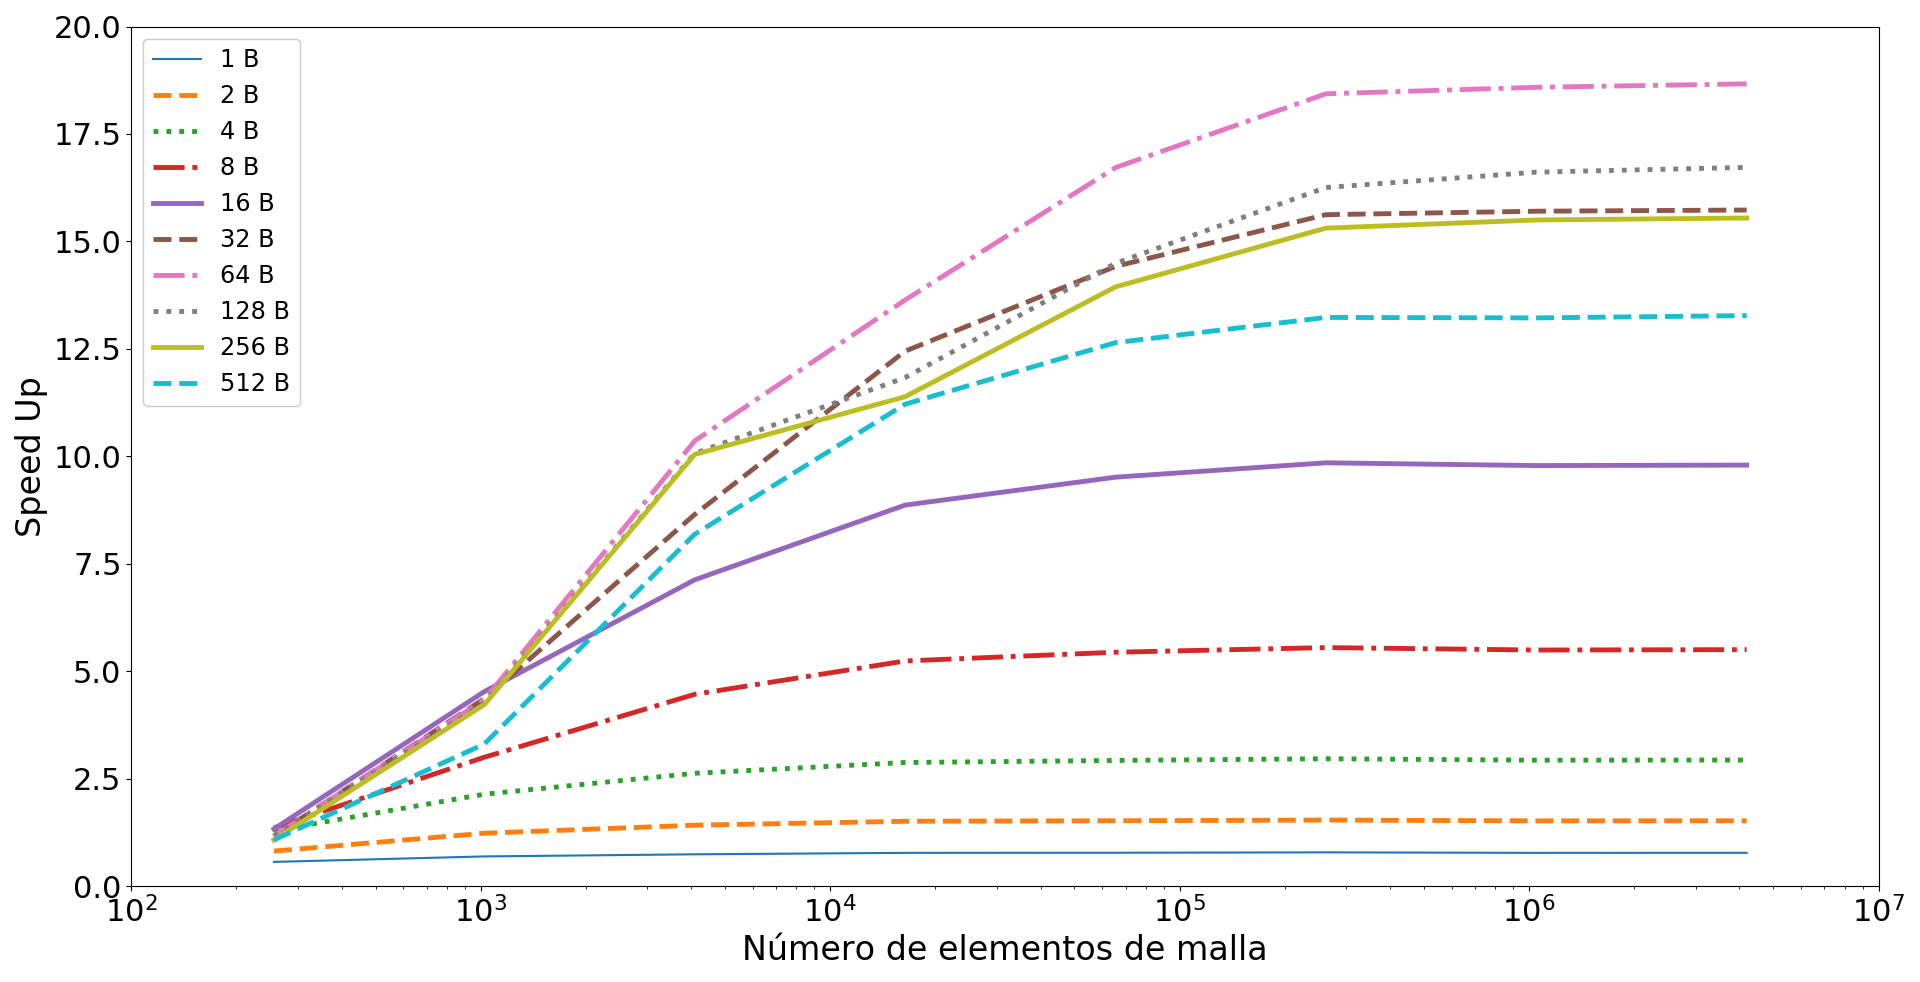
\includegraphics[width=\textwidth]{figs/cap4/s_760_MxC_simple_10}
	\caption{SU realizado para el problema de la Construcción de Maxwell en simple precisión con una CPU Intel Core i7-3770 y GPU NVIDIA GeForce GTX 760.} 
	\label{fig:s_760_MxC_simple_1.0}	
\end{figure}

\begin{figure}[htbp]
	\centering
	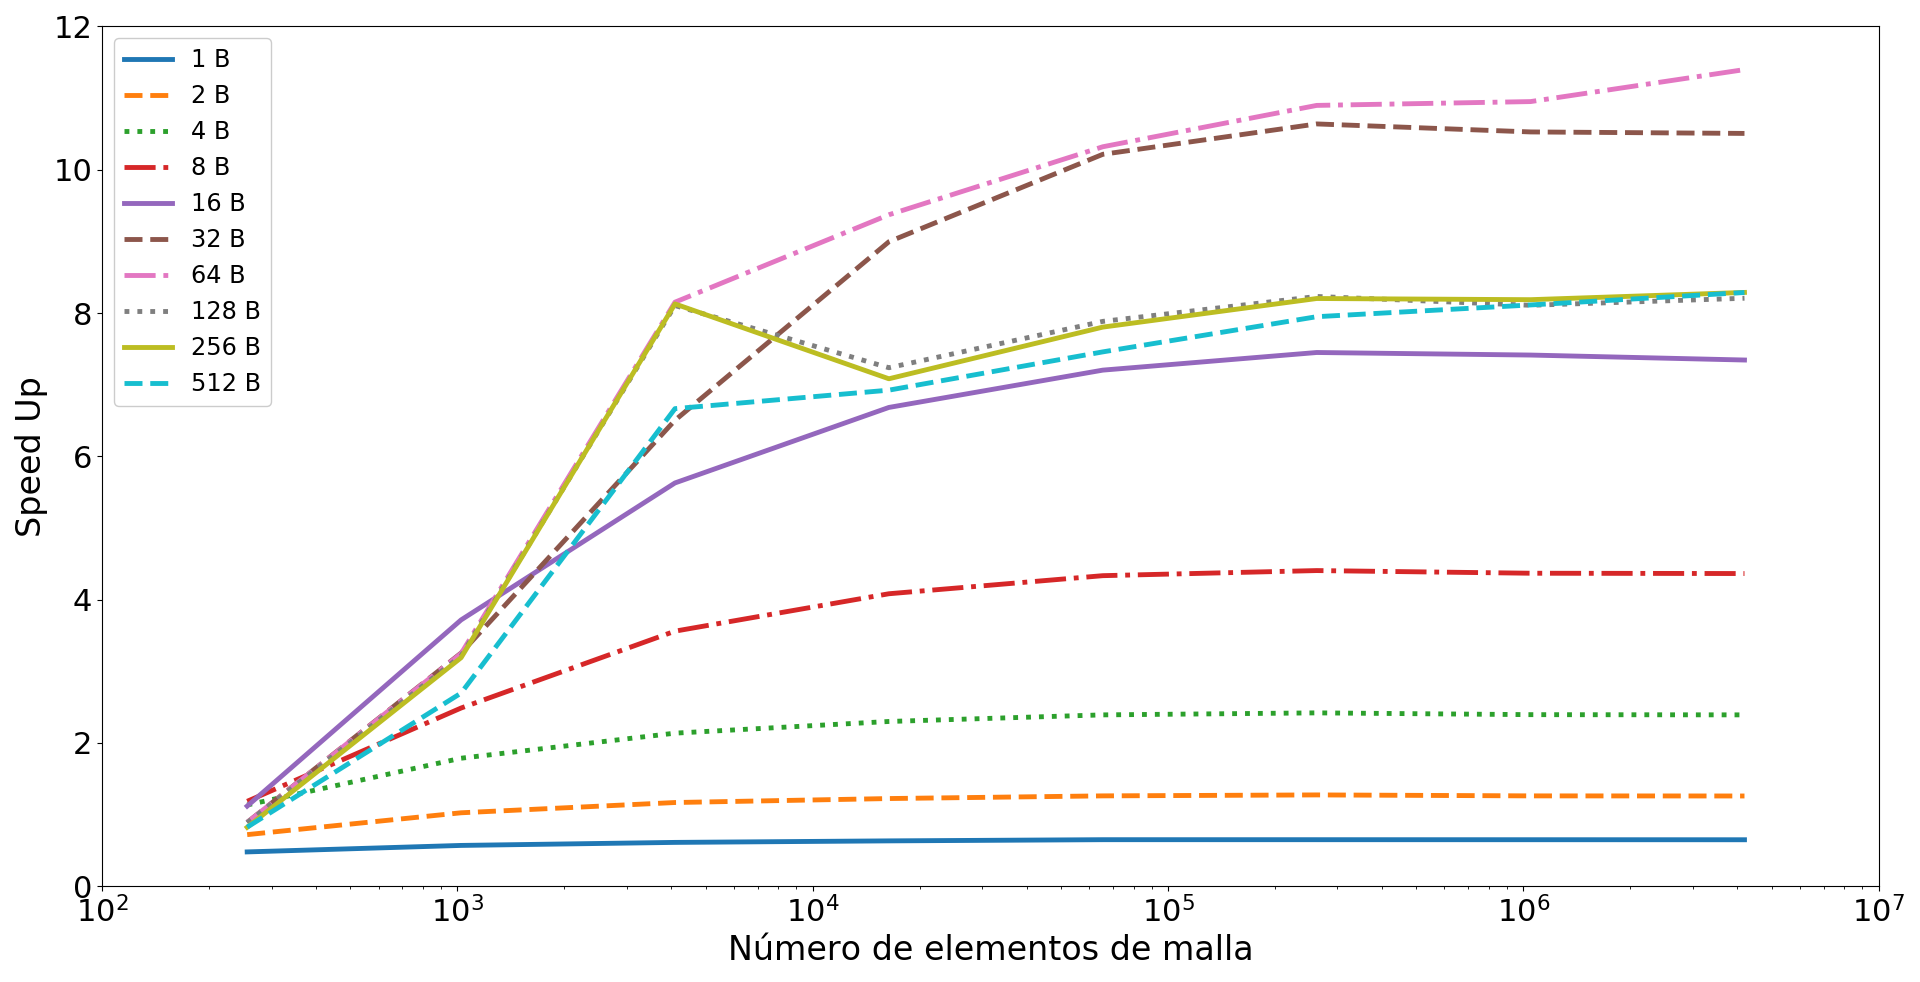
\includegraphics[width=\textwidth]{figs/cap4/s_760_MxC_double_10}
	\caption{SU realizado para el problema de la Construcción de Maxwell en doble precisión con una CPU Intel Core i7-3770 y GPU NVIDIA GeForce GTX 760.} 
	\label{fig:s_760_MxC_double_1.0}	
\end{figure}

\begin{figure}[h!]
	\centering
	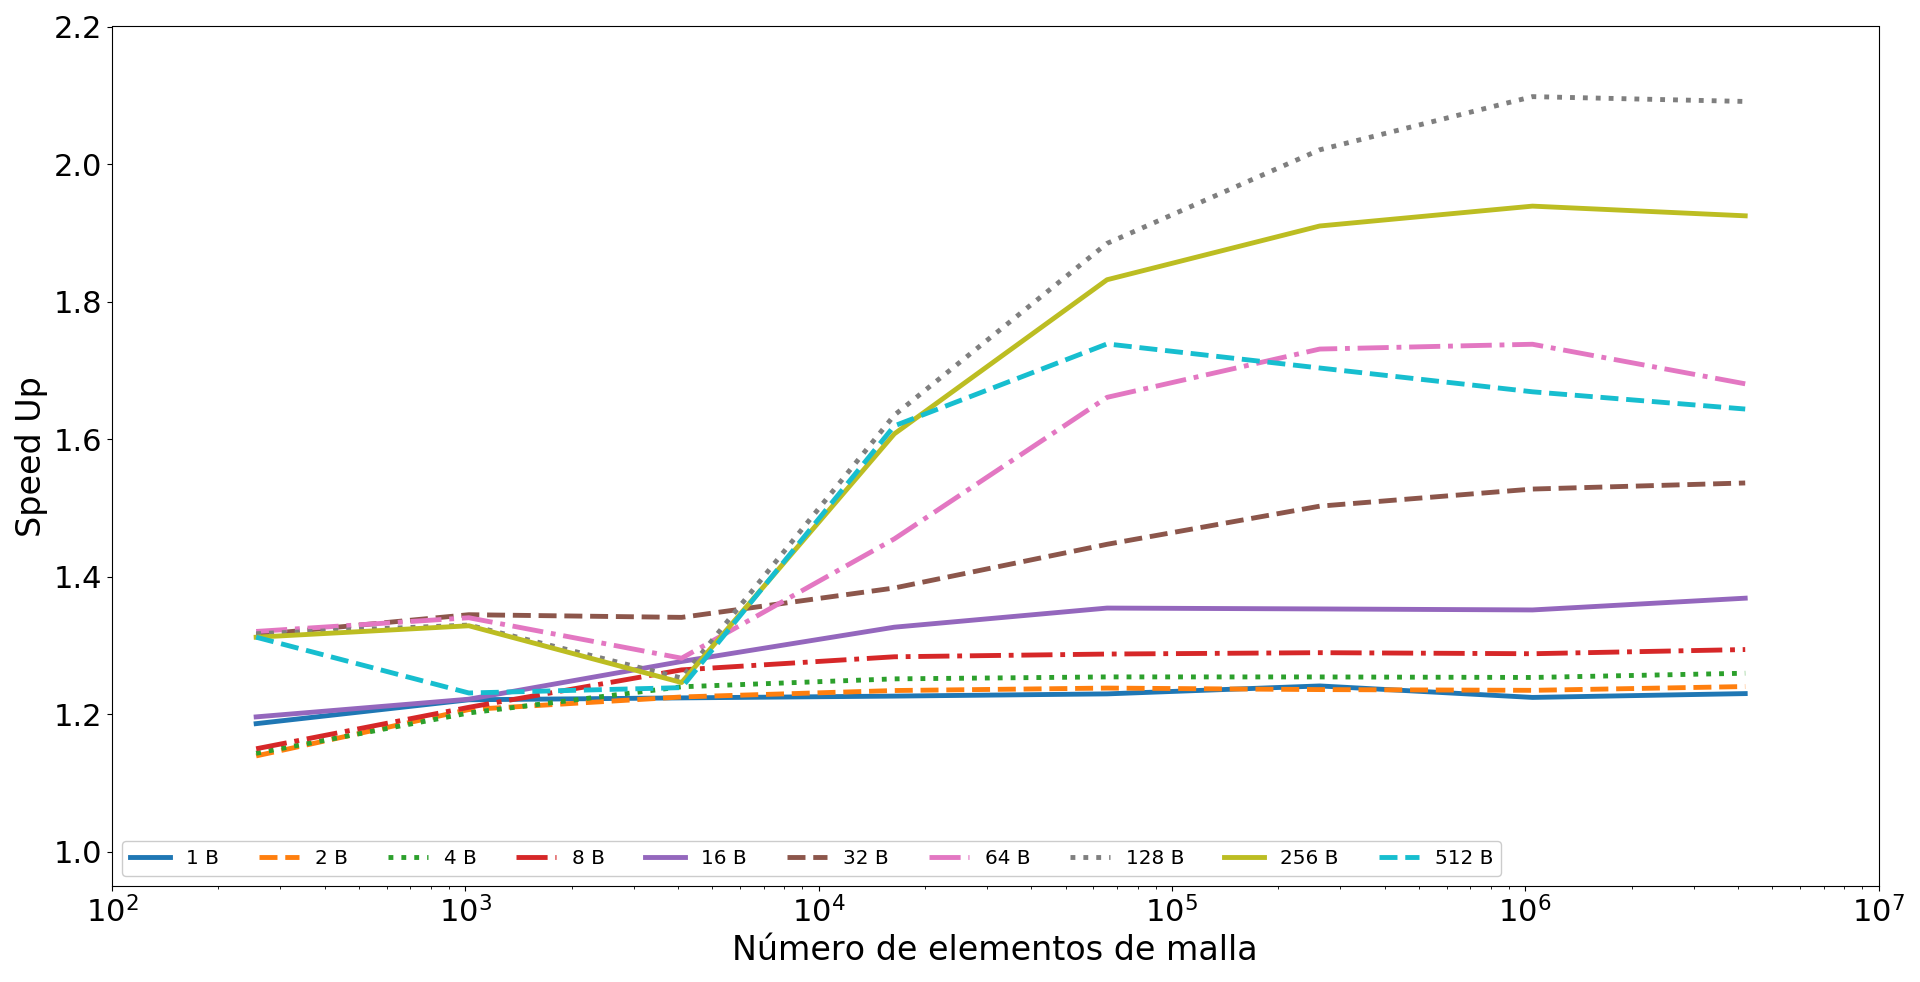
\includegraphics[width=\textwidth]{figs/cap4/c_760_MxC_cuda_10}
	\caption{$SU_p$ realizado para el problema de la Construcción de Maxwell en en el código de \textsc{Cuda C} con la GPU NVIDIA GeForce GTX 760.} 
	\label{fig:c_760_MxC_cuda_10}	
\end{figure}

La Figura (\ref{fig:c_760_MxC_cuda_10}) muestra el ${SU}_p$ del código de \textsc{Cuda C} en la GPU NVIDIA GeForce GTX 760. Para un número de \textit{thread block} igual a 64, el tiempo de cálculo en doble precisión es 1,68 veces mayor que en simple precisión en el mayor número de elementos de malla calculado. Se reporta únicamente el resultado para esa cantidad de \textit{thread block}, debido a que los resultados de las Figuras (\ref{fig:s_760_MxC_simple_1.0}) y (\ref{fig:s_760_MxC_double_1.0}) indican que es el que tiene un mayor SU.


\subsubsection{NVIDIA GeForce GTX 970}

Los tamaños de grilla que se utilizaron para realizar las pruebas de tiempo de esta placa, varían entre 16x16 nodos hasta 4096x4096 nodos en simple precisión y varían entre 16x16 nodos hasta 2048x2048 nodos en doble precisión . La cantidad de \textit{thread blocks} que se utilizó fueron de 1 a 512.



\begin{figure}[htbp]
	\centering
	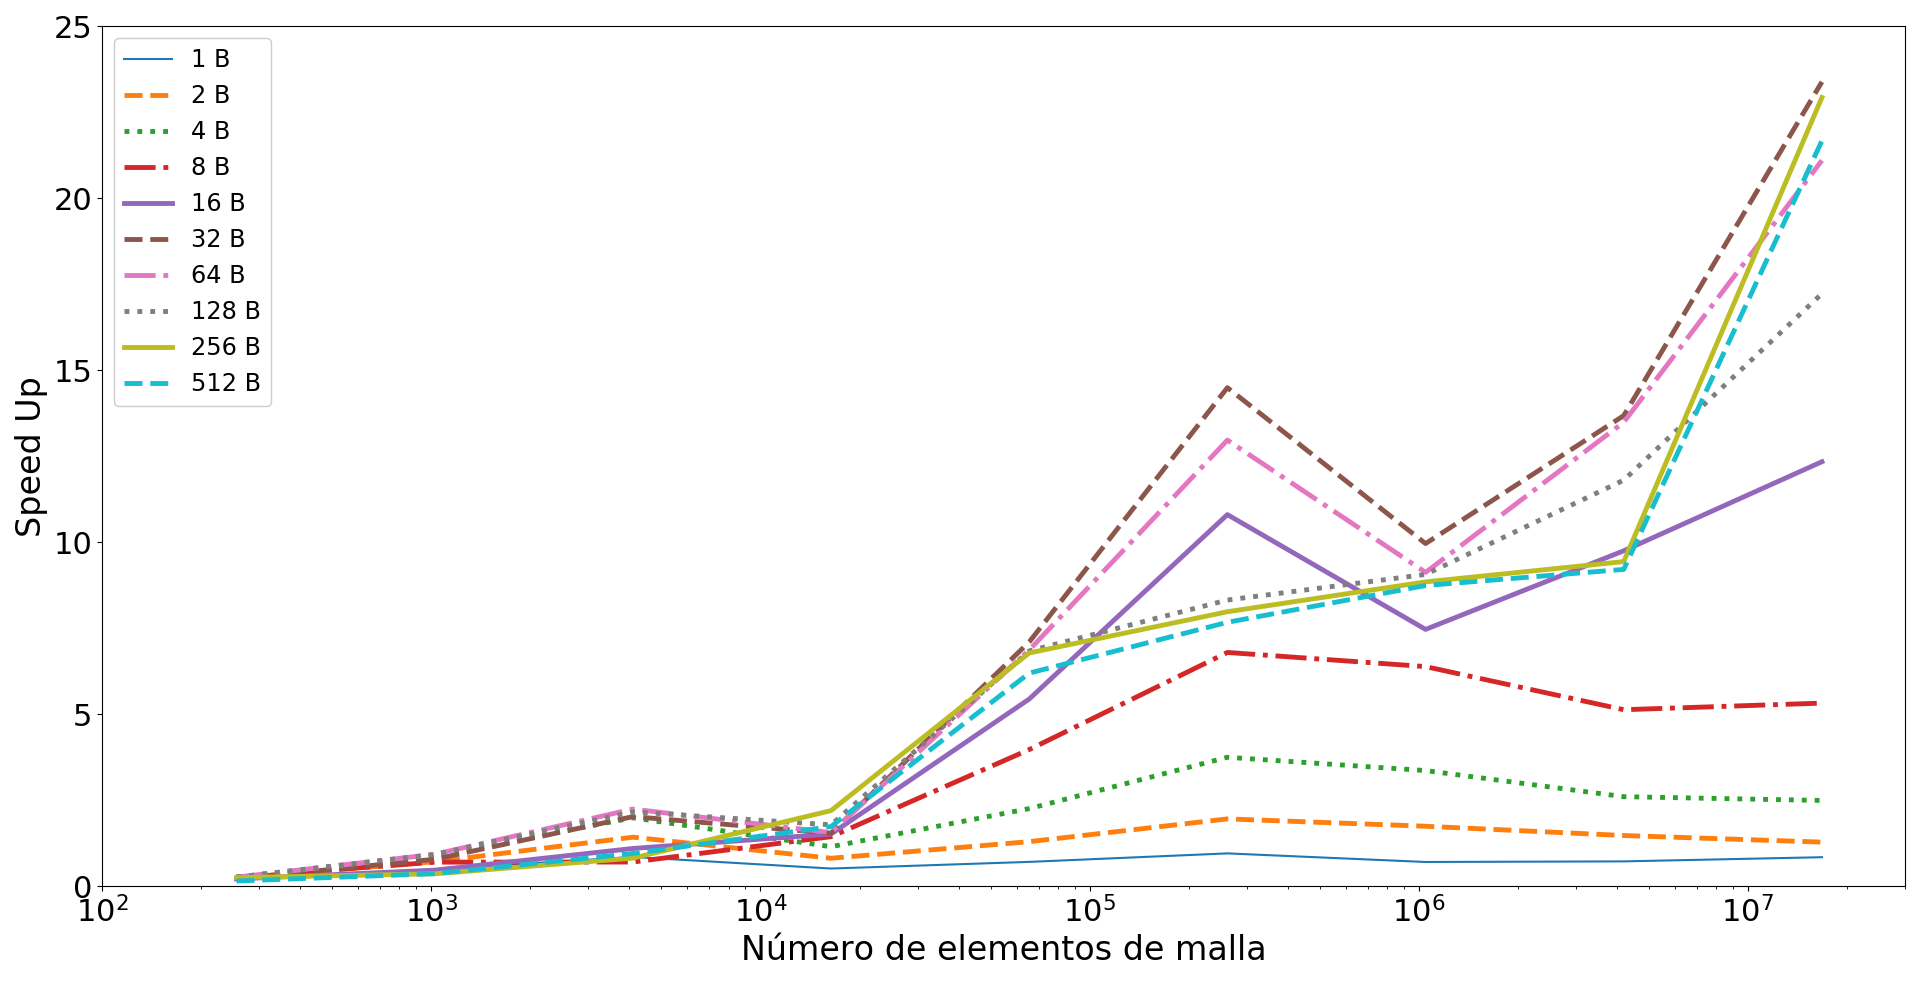
\includegraphics[width=0.99\textwidth]{figs/cap4/s_970_MxC_simple_10}
	\caption{SU realizado para el problema de la Construcción de Maxwell en simple precisión con una CPU Intel Core i7-4770 y GPU NVIDIA GeForce GTX 970.} 
	\label{fig:s_970_MxC_simple_10}	
\end{figure}

\begin{figure}[htbp]
	\centering
	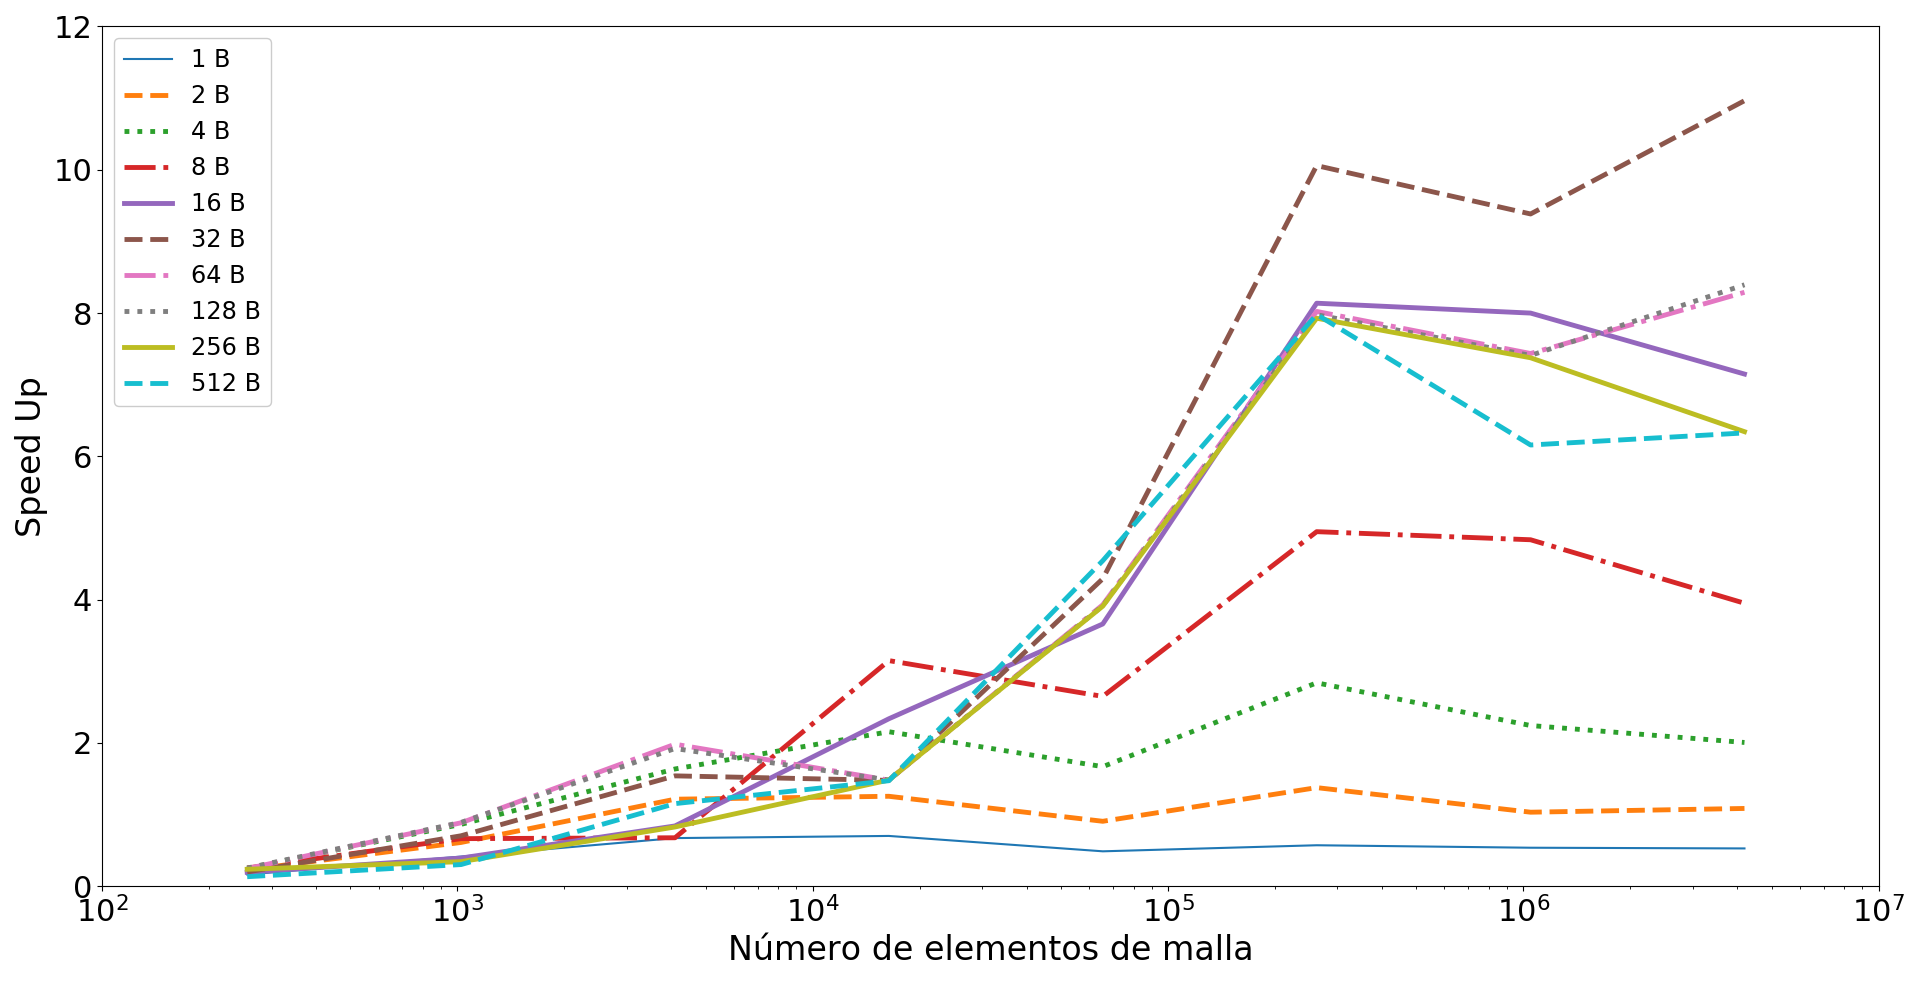
\includegraphics[width=0.99\textwidth]{figs/cap4/s_970_MxC_double_10}
	\caption{SU realizado para el problema de la Construcción de Maxwell en doble precisión con una CPU Intel Core i7-4770 y GPU NVIDIA GeForce GTX 970.} 
	\label{fig:s_970_MxC_double_10}	
\end{figure}

\newpage

Las Figuras (\ref{fig:s_970_MxC_simple_10}) y (\ref{fig:s_970_MxC_double_10}) muestran el SU obtenido en simple precisión y doble precisión respectivamente. El mejor resultado en ambos casos se obtuvo para un número de \textit{thread block} igual a 32, donde la mejora fue de 23.39 y 10.96 en simple y doble precisión respectivamente, para el mayor número de elementos de malla.

La Figura (\ref{fig:c_970_MxC_cuda_10}) muestra el ${SU}_p$ del código de \textsc{Cuda C} en la GPU NVIDIA GeForce GTX 970. Para un número de \textit{thread block} igual a 32, el tiempo de cálculo en doble precisión es 1,29 veces mayor que en simple precisión en el mayor número de elementos de malla calculado. Se reporta únicamente el resultado para esa cantidad de \textit{thread block}, debido a que los resultados de las Figuras (\ref{fig:s_970_MxC_simple_10}) y (\ref{fig:s_970_MxC_double_10}) indican que es el que tiene un mayor SU.

\begin{figure}[htbp]
	\centering
	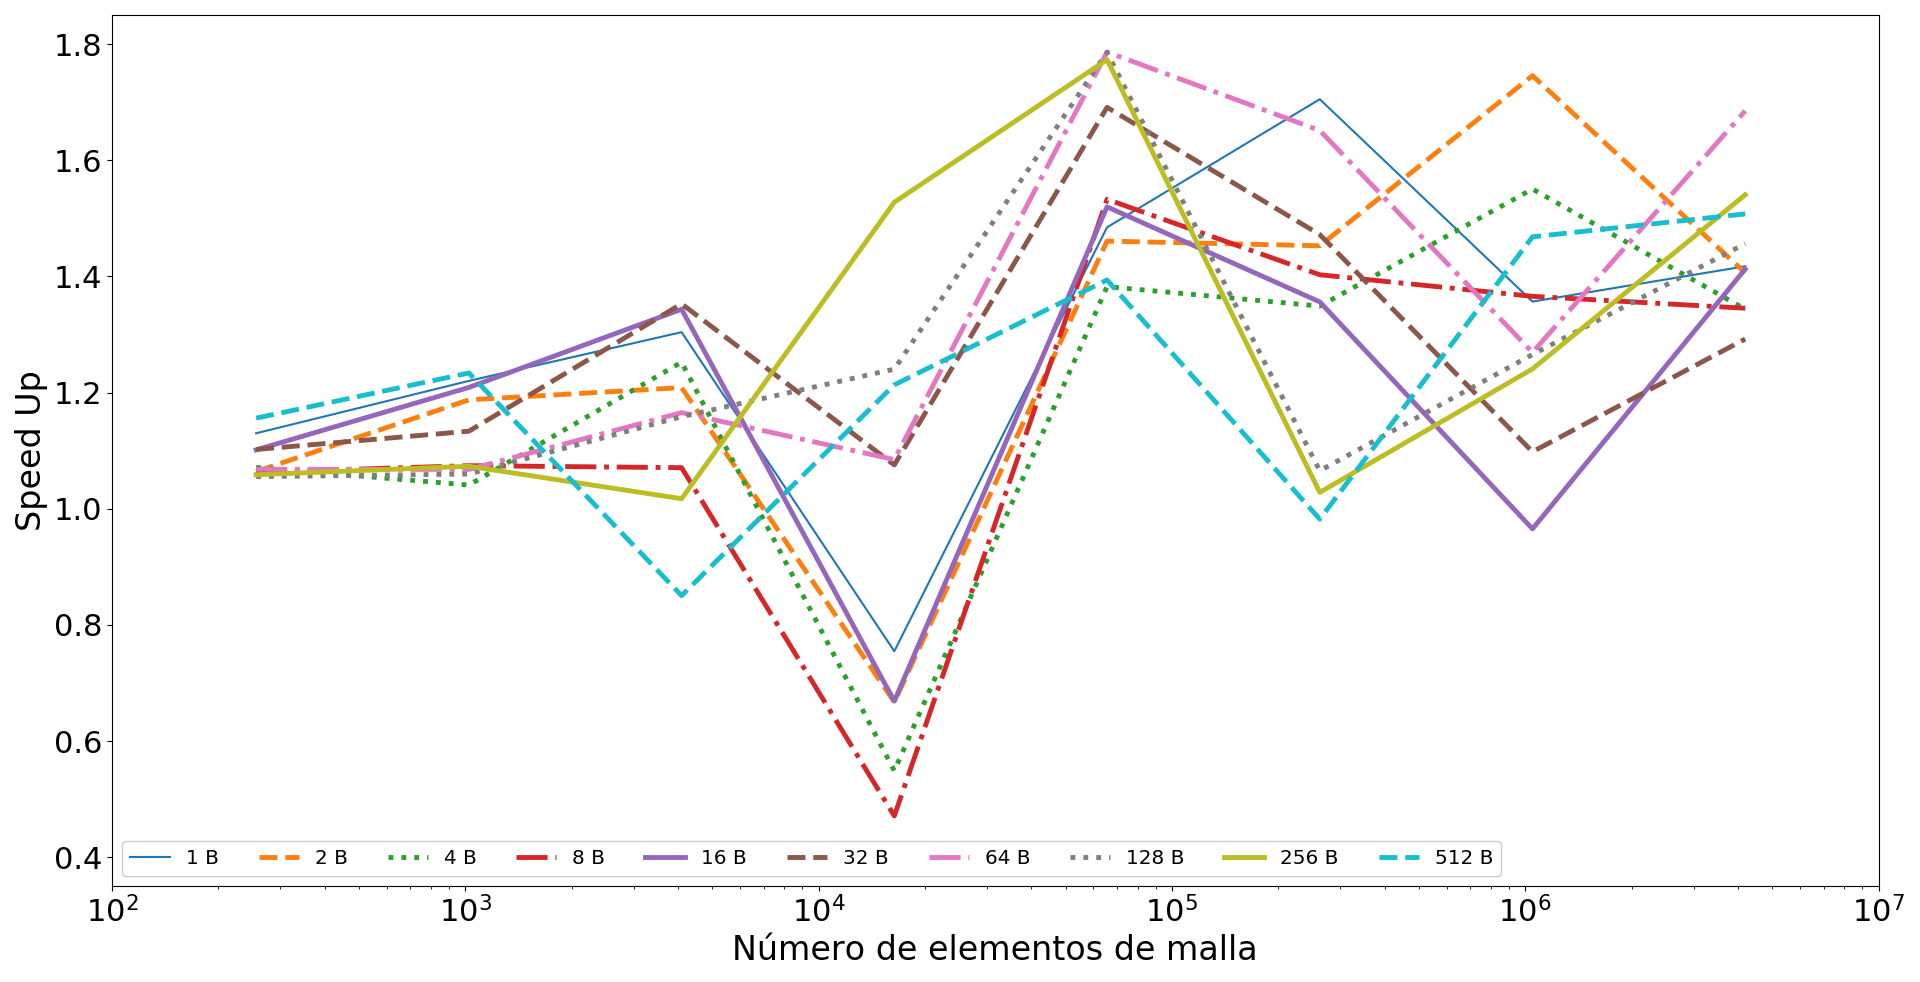
\includegraphics[width=\textwidth]{figs/cap4/c_970_MxC_cuda_10}
	\caption{$SU_p$ realizado para el problema de la Construcción de Maxwell en en el código de \textsc{Cuda C} con la GPU NVIDIA GeForce GTX 970.} 
	\label{fig:c_970_MxC_cuda_10}	
\end{figure}




Se puede concluir después de haber realizado un SU y $SU_p$ a las dos PC que se tuvo acceso para realizar el presente trabajo, de que la utilización de simple precisión en el código de \textsc{Cuda C} es más conveniente que doble precisión. Una de las razones es que no hay demasiada diferencia entre los valores que se pueden obtener, según los resultados obtenidos no difirieren más del 0,003 \%. Otra de las razones es que debido a las mejoras obtenidas en los tiempos de cálculo en las placas NVIDIA GeForce GTX 760 y NVIDIA GeForce GTX 970 en el código de \textsc{Cuda C} de 18.67 y 23.39 respectivamente en simple precisión que el código de \textsc{C}. Las mejoras en doble precisión de las ganancias son de 11.40 y 10.96 respectivamente en las placas mencionadas. Por lo que el resultado obtenido en simple precisión difiere apenas un 0.003 \% que en doble precisión, además siendo 1.68 y 1.29 veces más rapido según la GPU utilizada.

\newpage

\section{Estratificación de un fluido VdW con temperatura no uniforme (1D)}

\begin{figure}[htbp]
	\centering
	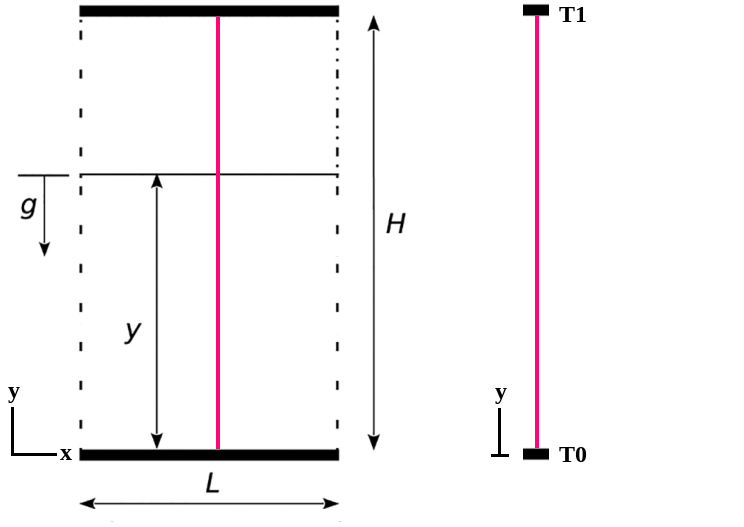
\includegraphics[width=0.7\textwidth]{figs/cap4/esquema_problema_VdW}
	\caption{Izquierda: Cavidad bidimensional de alto (H) y ancho (L), la linea vertical indica el problema unidimensional. Derecha: Cavidad unidimensional de alto (H). Ambas cavidades bajo la acción de la gravedad (g) y temperaturas fijas en los extremos de H.} 
	\label{fig:esquema_VdW}	
\end{figure}

Se quiere resolver el problema de una cavidad unidimensional en presencia de un fluido cuya EOS es la de Van der Waals; con temperatura  no uniforme y fuerza de gravedad no nula. Éste problema fue desarrollado por Berberan-Santos et al. \cite{berberan2002liquid} y extendido por Fogliatto et al. \cite{fogliatto2019simulation}. En este caso se resuelven las dos ecuaciones pseudo-potencial del LBM, la ecuación hidrodinámica y la ecuación de energía.

Se toma como coordenada del problema \textit{y}, teniéndose una temperatura fija $T_{0}$ en $y = 0$ y $T_{1}$ en $y = H$ como se observa en el panel derecho de la Figura (\ref{fig:esquema_VdW}) en presencia de la gravedad.

El gradiente de presión surge de realizar el balance de momento en un volumen diferencial, obteniéndose:

\begin{align}
	\frac{d P}{d y} = - g M C(y)
\end{align}

siendo \textit{g} la gravedad, \textit{M} el peso molecular, $C = \frac{1}{v}$ la fracción molar, \textit{v} el volumen molar y \textit{P} la presión.

Realizando la adimensionalización $ P_r = \frac{P}{P_c}$ , $ T_r = \frac{T}{T_c}$, $c = C v_c$ y $E_r = \frac{M g y}{R T_c}$; siendo \textit{c} el punto crítico en el cuál comienza la coexistencia de las dos fases, se pueden reemplazar en el gradiente de presión una ecuación de estado para obtener una ecuación adimensional con la concentración molar distribuida \cite{fogliatto2019simulation}.



En particular, para la EOS de VdW se obtiene:

\begin{align}
	\frac{d c}{d E_r} = - \left[ c + \frac{d T_r}{d E_r} \left( \frac{c}{1 - \frac{c}{3}}\right) \right] \left[	\frac{1}{\frac{T_r}{{\left(1- \frac{c}{3}\right)}^2} - \frac{9}{4} c}  \right] 
	\label{eq:adim_dif}
\end{align} 

donde la posición de la interface dentro de la cavidad se puede determinar utilizando la masa inicial, siendo la misma una condición inicial para realizar la integración de la Ec. (\ref{eq:adim_dif}). Si se elige  resolver iterativamente la Ec. (\ref{eq:adim_dif}) junto con la ecuación macroscópica Ec. (\ref{eq:calor_ecu}) (ecuación del calor) se puede obtener las distribuciones de densidad y temperatura de la cavidad \cite{fogliatto2019simulation}. A partir de la densidad y temperatura recuperadas, se obtienen dos curvas adimensionales correspondientes al perfil de temperatura y al de concentraciones. 

En éste problema a validar, se toma como temperatura fija $T_1 = 0.99 \> T_c$, y se hace variar el valor de  $T_0$. Se asigna la siguiente nomenclatura $\rho_r = \frac{\rho}{\rho_c}$ y  $Y_r = \frac{y}{H}$, que en este caso coinciden con $c$ y $\frac{E_r}{E_{r_{max}}}$ respectivamente. En las Figuras (\ref{fig:v_760_VdW_c_simple_rho_y}) y (\ref{fig:v_760_VdW_c_simple_T_y}) se muestran las curvas adimensionales de $ \rho_r - Y_r $ y $ T_r - Y_r $ respectivamente.
\newline
\subsection{Validación}

La validación de este problema se hizo utilizando los parámetros $a =0,5$ y $b = 4,0$; para un tamaño de malla de 3 x 300 nodos y $T_0 = T_r$, con $T_r = 0,6 ; 0,7 ; 0,8 \> y \> 0,9$.  Los parámetros de LBM son los que se detallan a continuación:
\begin{align*}
\centering
diag(\mathbf{\Lambda}) & = 
\begin{bmatrix}
1.0 & 0.8 & 1.1 & 1.0 & 1.1 & 1.0 & 1.1 & 0.8 & 0.8 \\
\end{bmatrix}\\
diag(\mathbf{Q}) & = 
\begin{bmatrix}
1.0 & 1.0 & 1.0 & 0.8 & 1.0 & 0.8 & 1.0 & 1.0 & 1.0 \\
\end{bmatrix}\\
\alpha_{1} & = 1.0 \qquad 	\alpha_{2} = 1.0 \qquad C_{v} = 1.0\\
G & = -1.0 \quad c = 1.0 \quad \sigma = 0.125 \quad a = 0.5 \quad b = 4.0 \\
\mathbf{g} & = (0.0 \quad-1.234567e^{-7}\quad 0.0 ) \qquad \rho_c = \frac{1}{12} \qquad T_c = 0.037037037
\end{align*}
Las Figuras (\ref{fig:v_760_VdW_c_simple_rho_y}) y (\ref{fig:v_760_VdW_c_simple_T_y})  muestran la validación del código realizado en \textsc{C} para simple precisión en una GPU NVIDIA GeForce GTX 760 con distintos valores de $T_0$. 

El quiebre abrupto y discontinuo de la densidad a lo largo de la columna en la Figura (\ref{fig:v_760_VdW_c_simple_rho_y}) muestra la coexistencia de las dos fases, para la solución analítica. Debido a que se tiene una solución continua y difusa porque el modelo toma una cierta cantidad de nodos como separación entre ambas fases, se presenta una mayor diferencia en el ajuste de la curva obtenida con la analítica en el cambio de fase. Lo mismo sucede en la Figura (\ref{fig:v_760_VdW_c_simple_T_y}). En todos los casos se simularon 750000 pasos de tiempo hasta alcanzar una solución estacionaria. El resultado obtenido para ambas curvas validades es similar en primer orden en el código de \textsc{C} y \textsc{Cuda C}.

\begin{figure}[h!]
	\centering
	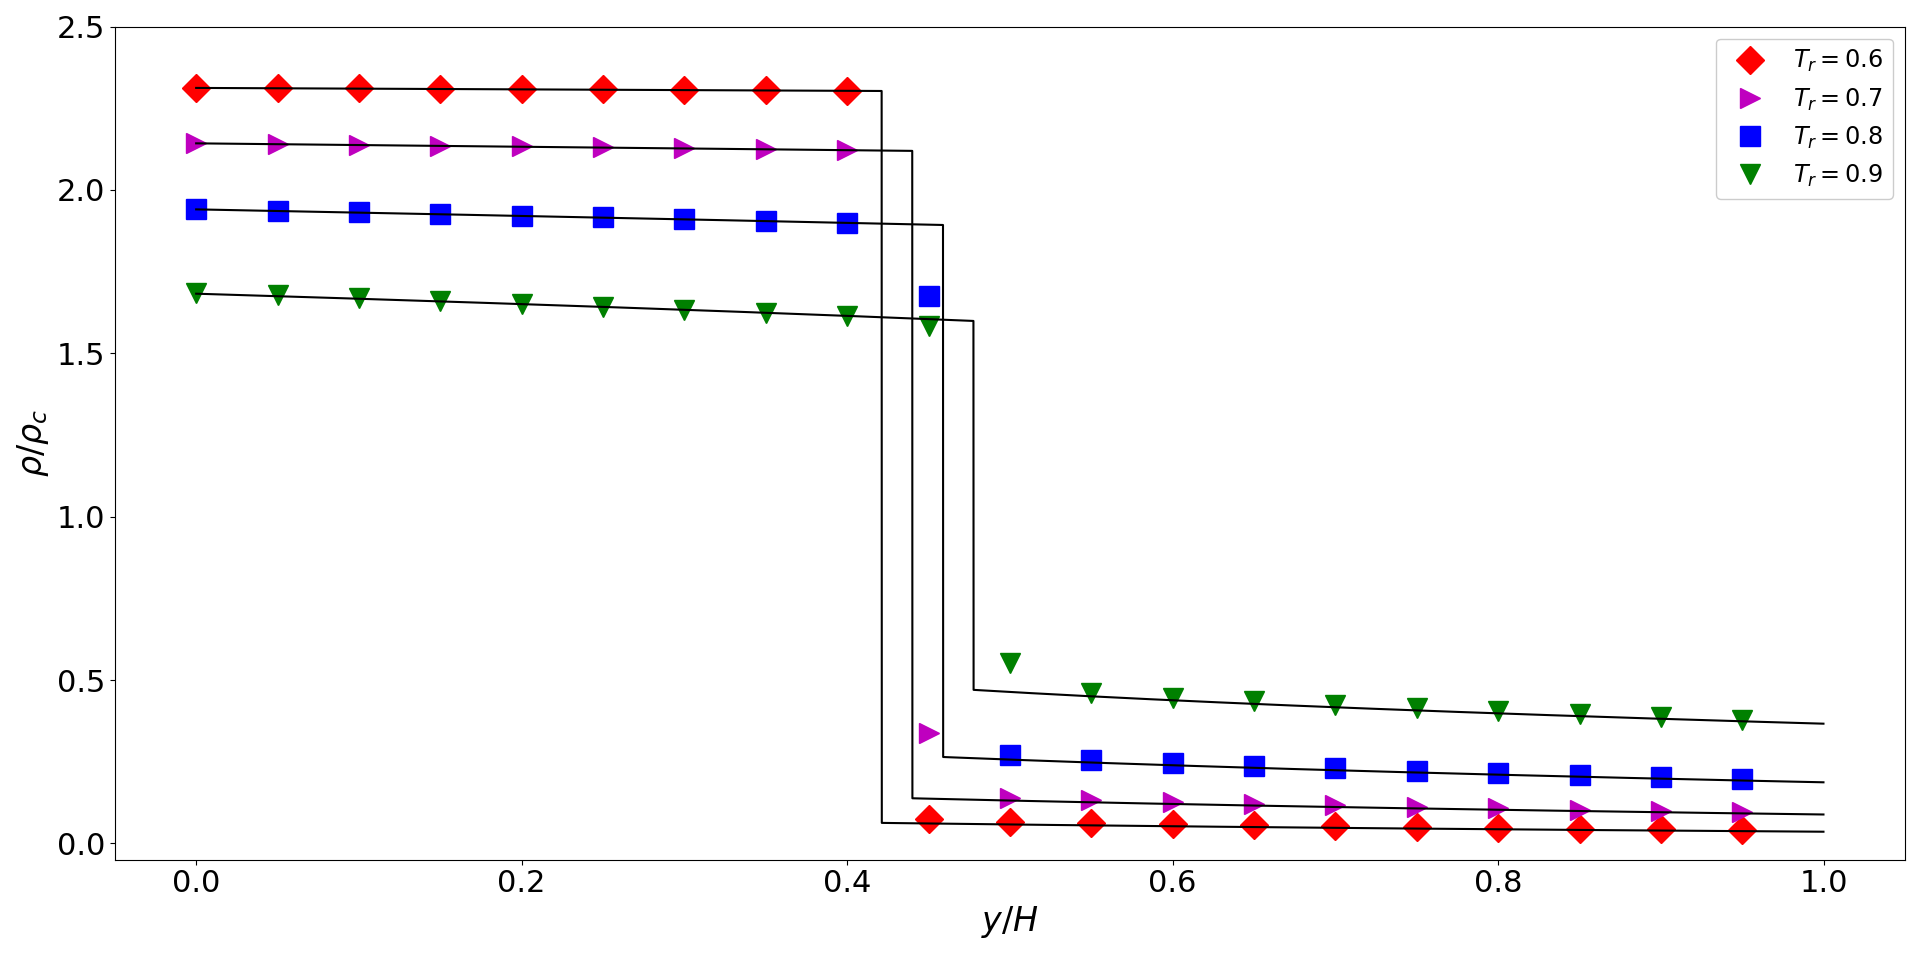
\includegraphics[width=\textwidth]{figs/cap4/v_760_VdW_c_simple_rho_y}
	\caption{Perfil de densidad adimensional a lo largo de la cavidad, para valores de $T_0 = T_r$, siendo $T_r = 0,6\> ;\> 0,7\> ;\> 0,8\>\> y\>\> 0,9$, para un fluido de VdW con los parámetros $a = 0,5 $ y $b = 4,0 $, obtenida en simple precisión en la GPU NVIDIA GeForce GTX 760 en el código desarrollado en \textsc{C}.}
	\label{fig:v_760_VdW_c_simple_rho_y}	
\end{figure}

\begin{figure}[h!]
	\centering
	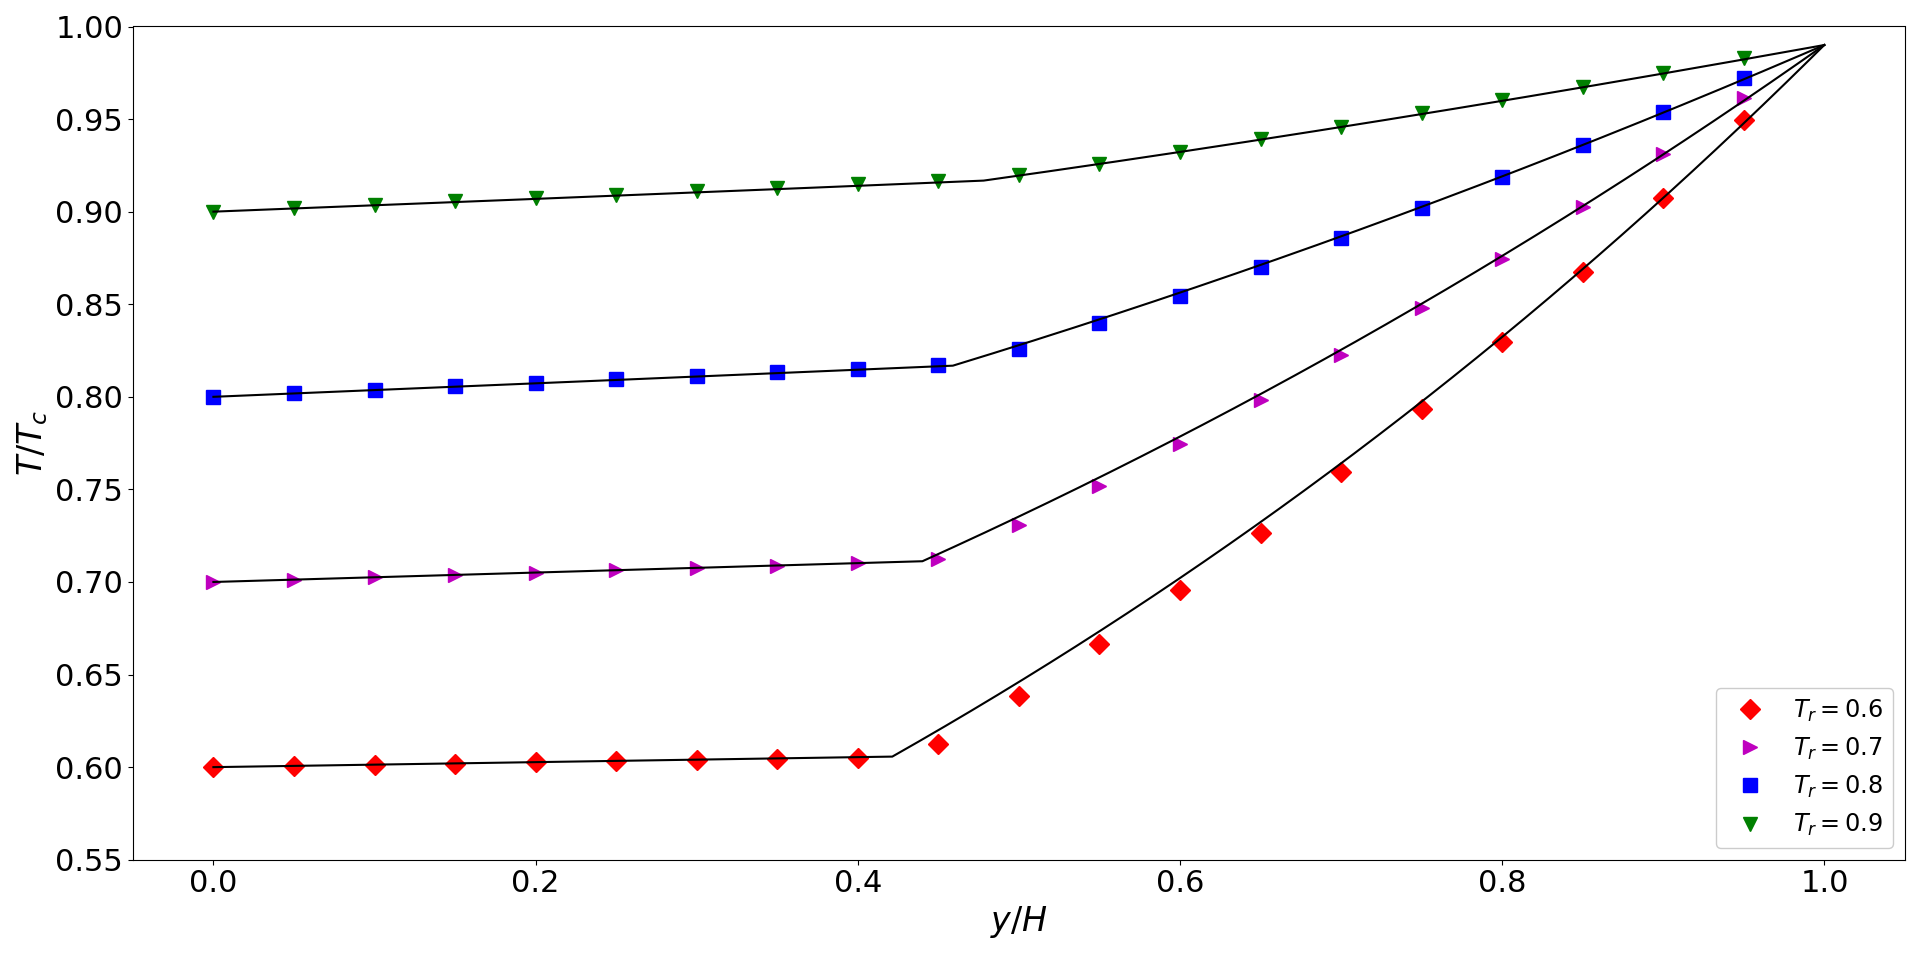
\includegraphics[width=\textwidth]{figs/cap4/v_760_VdW_c_simple_T_y}
	\caption{Perfil de temperatura adimensional a lo largo de la cavidad de la pared, para valores de $T_0 = T_r$, siendo $T_r = 0,6\> ;\> 0,7\> ;\> 0,8\>\> y\>\> 0,9$, para un fluido de VdW con los parámetros $a = 0,5 $ y $b = 4,0 $, obtenida en simple precisión en la GPU NVIDIA GeForce GTX 760 en el código desarrollado en \textsc{C}.}
	\label{fig:v_760_VdW_c_simple_T_y}	
\end{figure}

\newpage

\subsection{Speed Up}

En la presente sección se muestran las mejoras en el tiempo de cálculo realizados para el código de \textsc{C} y \textsc{Cuda C}. El índice que se utiliza es el SU y $SU_p$ como indica la Ec. (\ref{eq:speedup}). Se tomó una $T_r$ fija y se varió el tamaño de la grilla, de manera que ésta siempre tuviese una altura constante de 300 nodos y variando la dimensión en el eje \textsc{X} respetando un número de nodos de potencia de 2 (exceptuando el primer valor que es 3) . La cantidad de \textit{thread blocks} que se utilizó para realizar la comnparación en el código de \textsc{CUDA} fueron de potencia de 2.

\subsubsection{NVIDIA GeForce GTX 760}

Los tamaños de grilla que se utilizaron para realizar las pruebas de tiempo de esta placa, varían entre 3x300 nodos hasta 1638400x300 nodos. La cantidad de \textit{thread blocks} que se utilizó fueron de 1 a 512.

Las Figuras (\ref{fig:s_760_VdW_simple_10}) y (\ref{fig:s_760_VdW_double_10}) muestran el SU obtenido en simple y doble precisión respectivamente. El mejor resultado en ambos casos se obtuvo para un número de \textit{thread block} igual a 64, donde la mejora fue de 13.26 y 7.88 en simple y doble precisión respectivamente, para el mayor número de elementos de malla.



\begin{figure}[htbp]
	\centering
	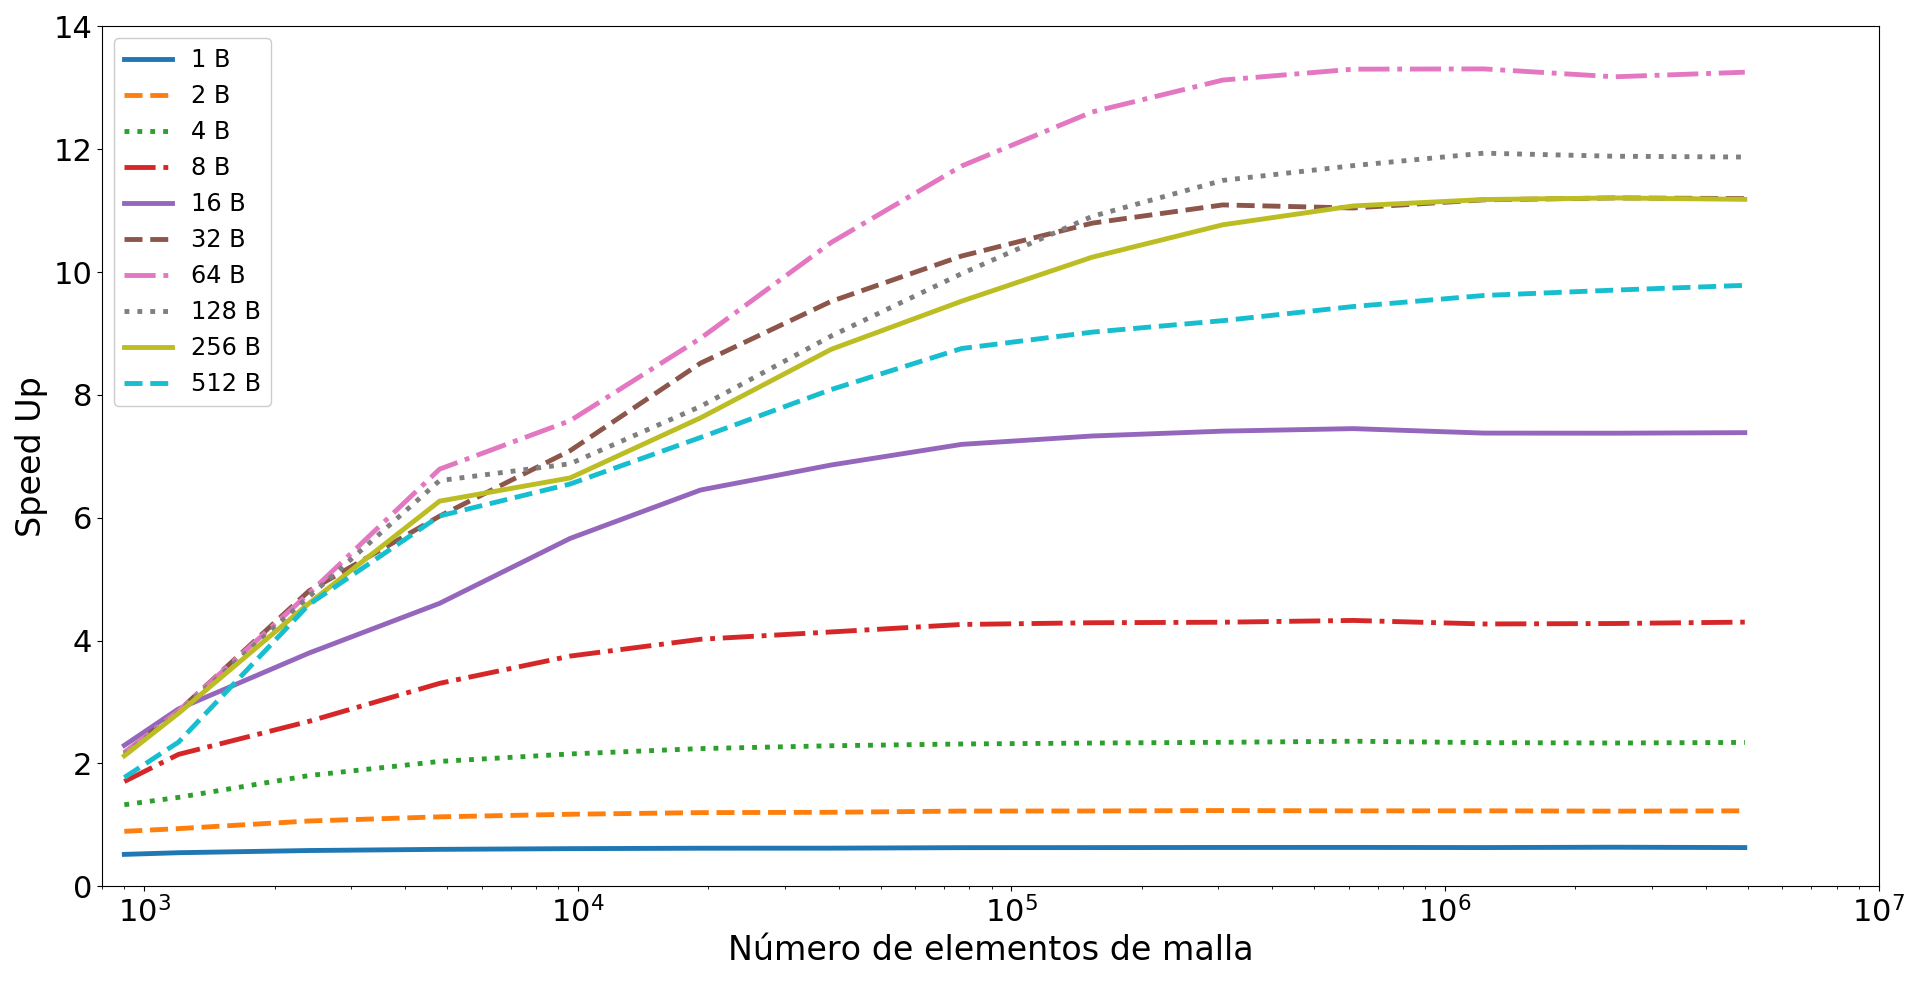
\includegraphics[width=\textwidth]{figs/cap4/s_760_VdW_simple_10}
	\caption{SU realizado para el problema de la Estratificación de un fluido Van dar Waals en simple precisión con una CPU Intel Core i7-3770 y GPU NVIDIA GeForce GTX 760.} 
	\label{fig:s_760_VdW_simple_10}	
\end{figure}

\begin{figure}[htbp]
	\centering
	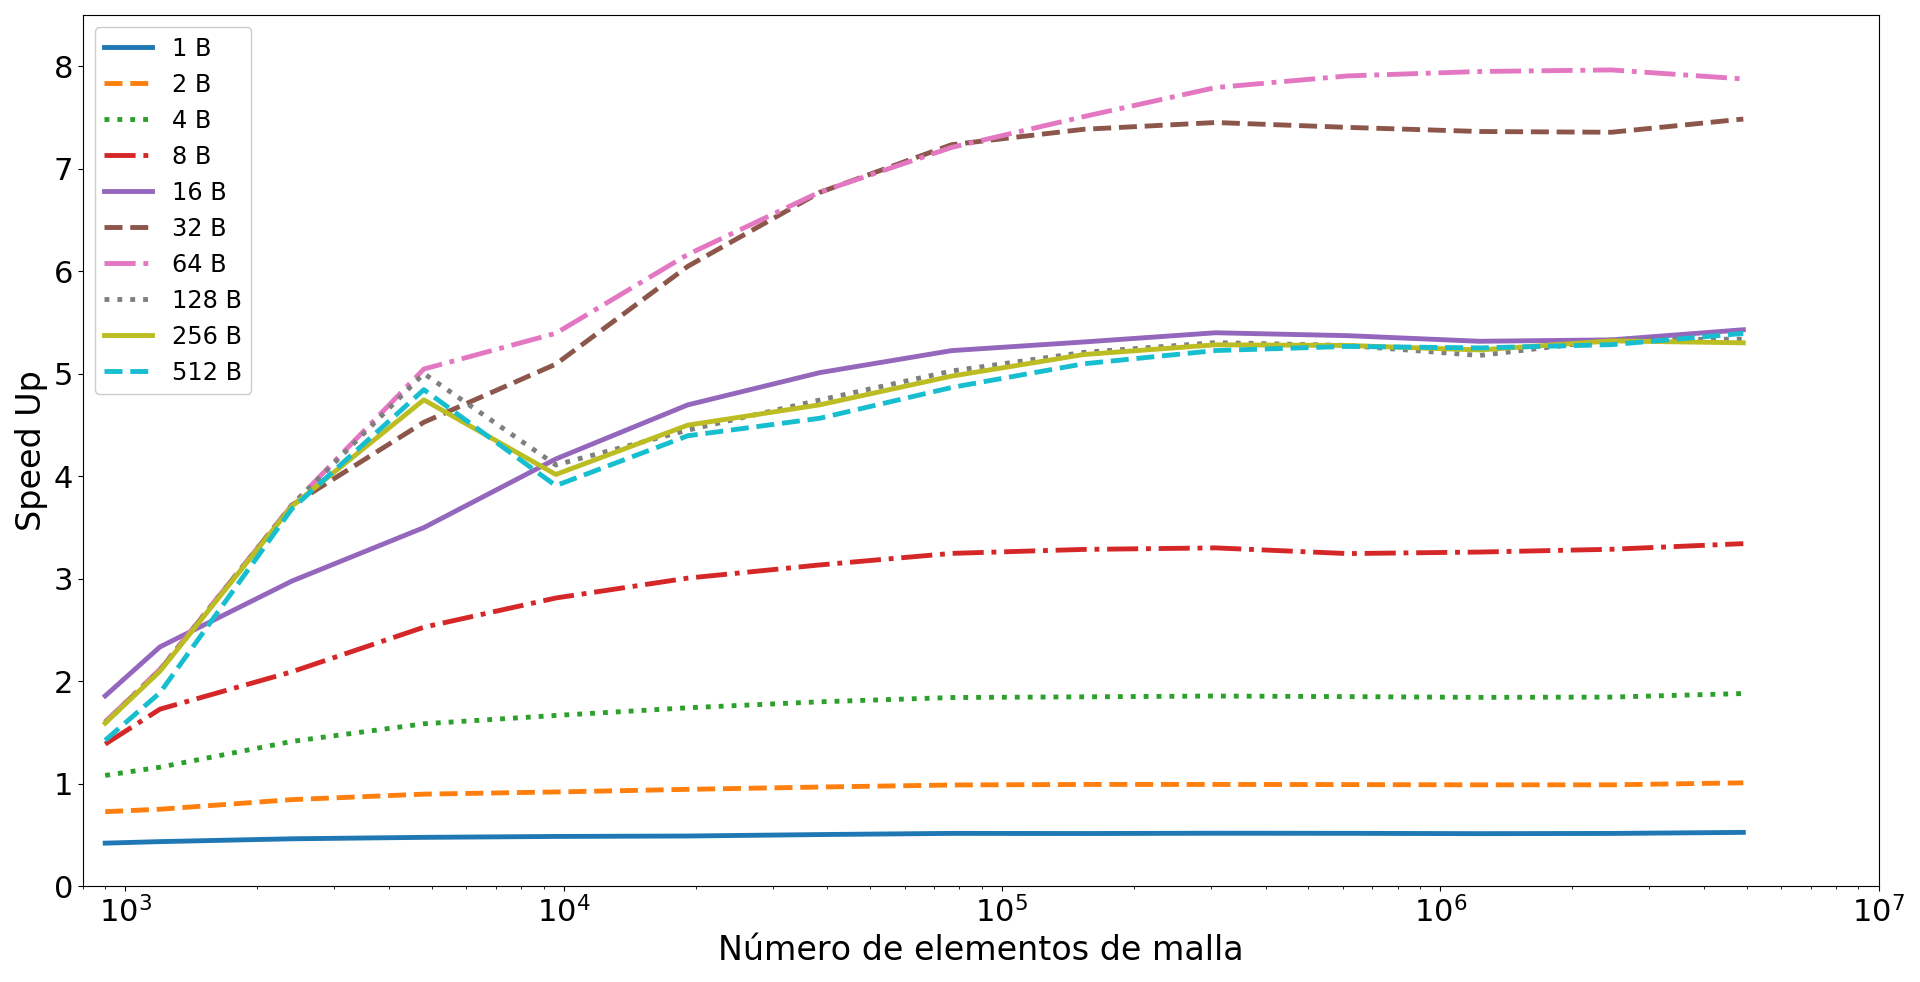
\includegraphics[width=\textwidth]{figs/cap4/s_760_VdW_double_10}
	\caption{SU realizado para el problema de la Estratificación de un fluido Van dar Waals en doble precisión con una CPU Intel Core i7-3770 y GPU NVIDIA GeForce GTX 760.} 
	\label{fig:s_760_VdW_double_10}	
\end{figure}

La Figura (\ref{fig:c_760_VdW_cuda_10}) muestra el ${SU}_p$ del código de \textsc{Cuda C} en la GPU NVIDIA GeForce GTX 760. Para un número de \textit{thread block} igual a 64, el tiempo de cálculo en doble precisión es 1,77 veces mayor que en simple precisión en el mayor número de elementos de malla calculado. Se reporta únicamente el resultado para esa cantidad de \textit{thread block}, debido a que los resultados anteriores indican que es el que tiene un mayor SU.

\begin{figure}[h!]
	\centering
	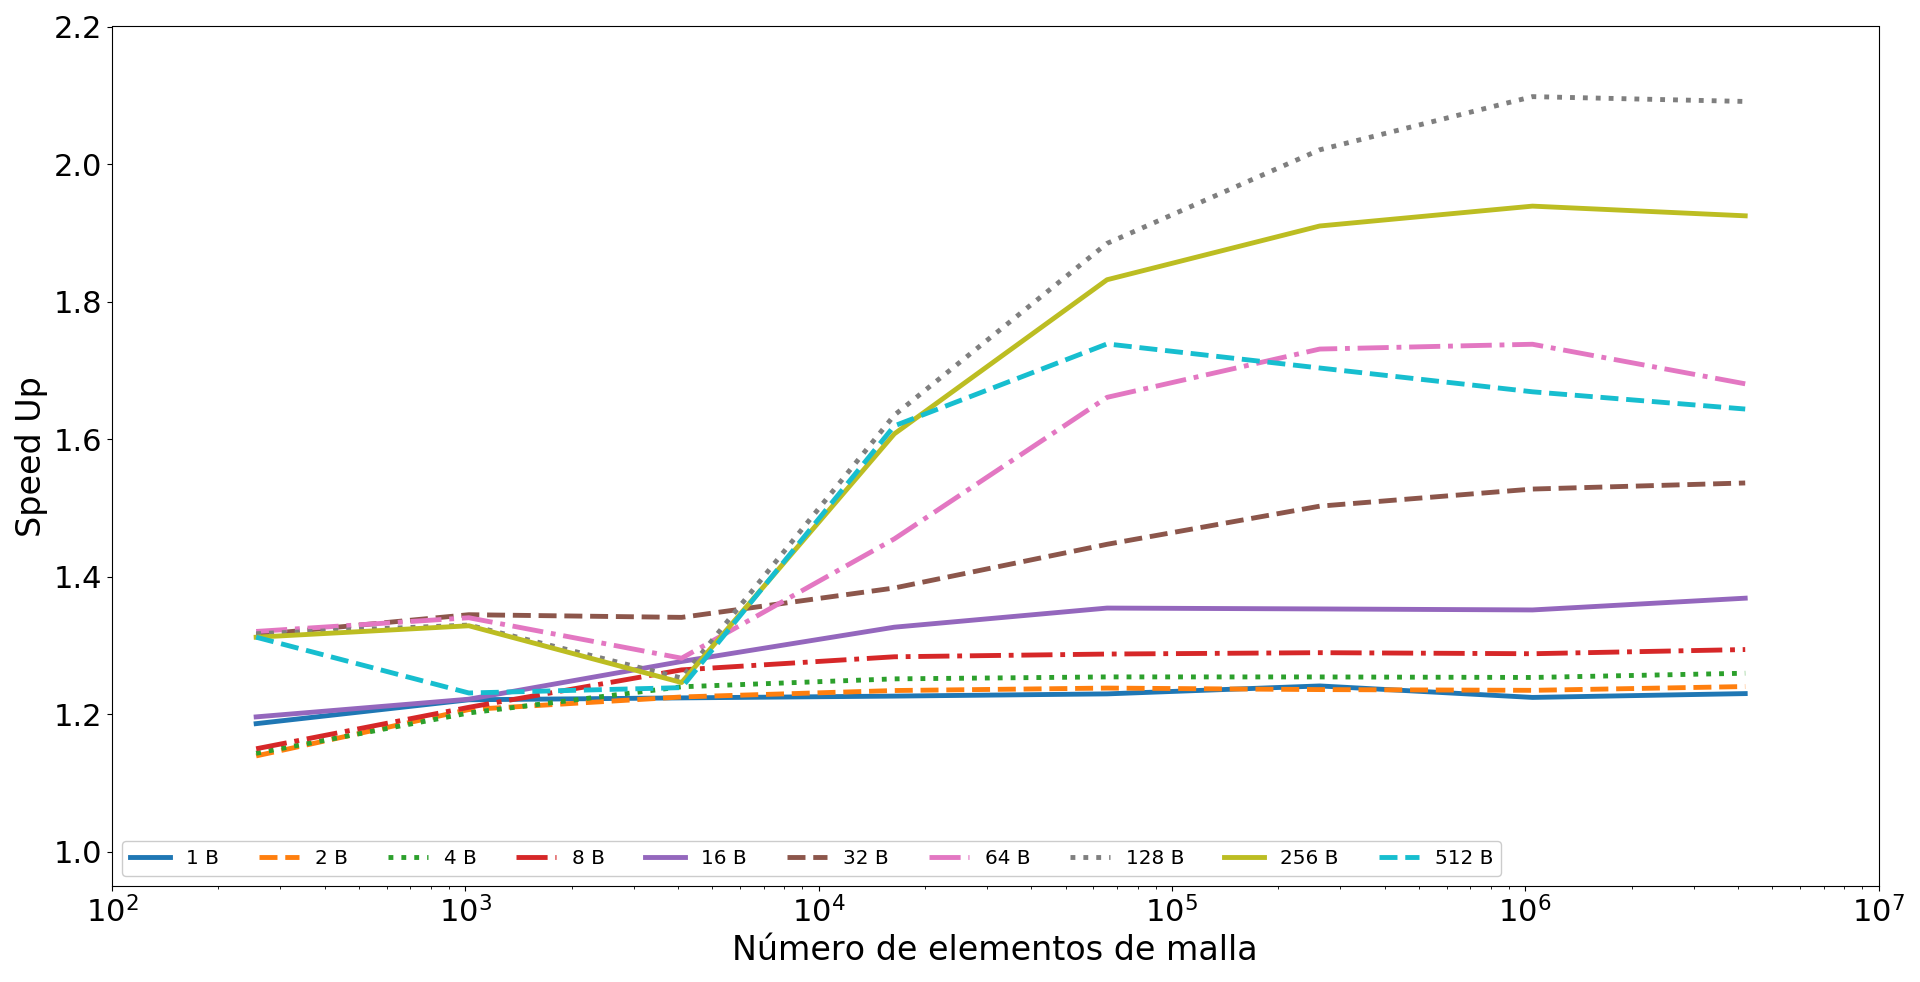
\includegraphics[width=\textwidth]{figs/cap4/c_760_MxC_cuda_10}
	\caption{$SU_p$ realizado para el problema de la Estratificación de un fluido Van der Waals en en el código de \textsc{Cuda C} con la GPU NVIDIA GeForce GTX 760.} 
	\label{fig:c_760_VdW_cuda_10}	
\end{figure}

\newpage

\subsubsection{NVIDIA GeForce GTX 970}

Los tamaños de grilla que se utilizaron para realizar las pruebas de tiempo de esta placa, varían entre 3x300 nodos hasta 1638400x300 nodos. La cantidad de \textit{thread blocks} que se utilizó fueron de 1 a 512.


\begin{figure}[h!]
	\centering
	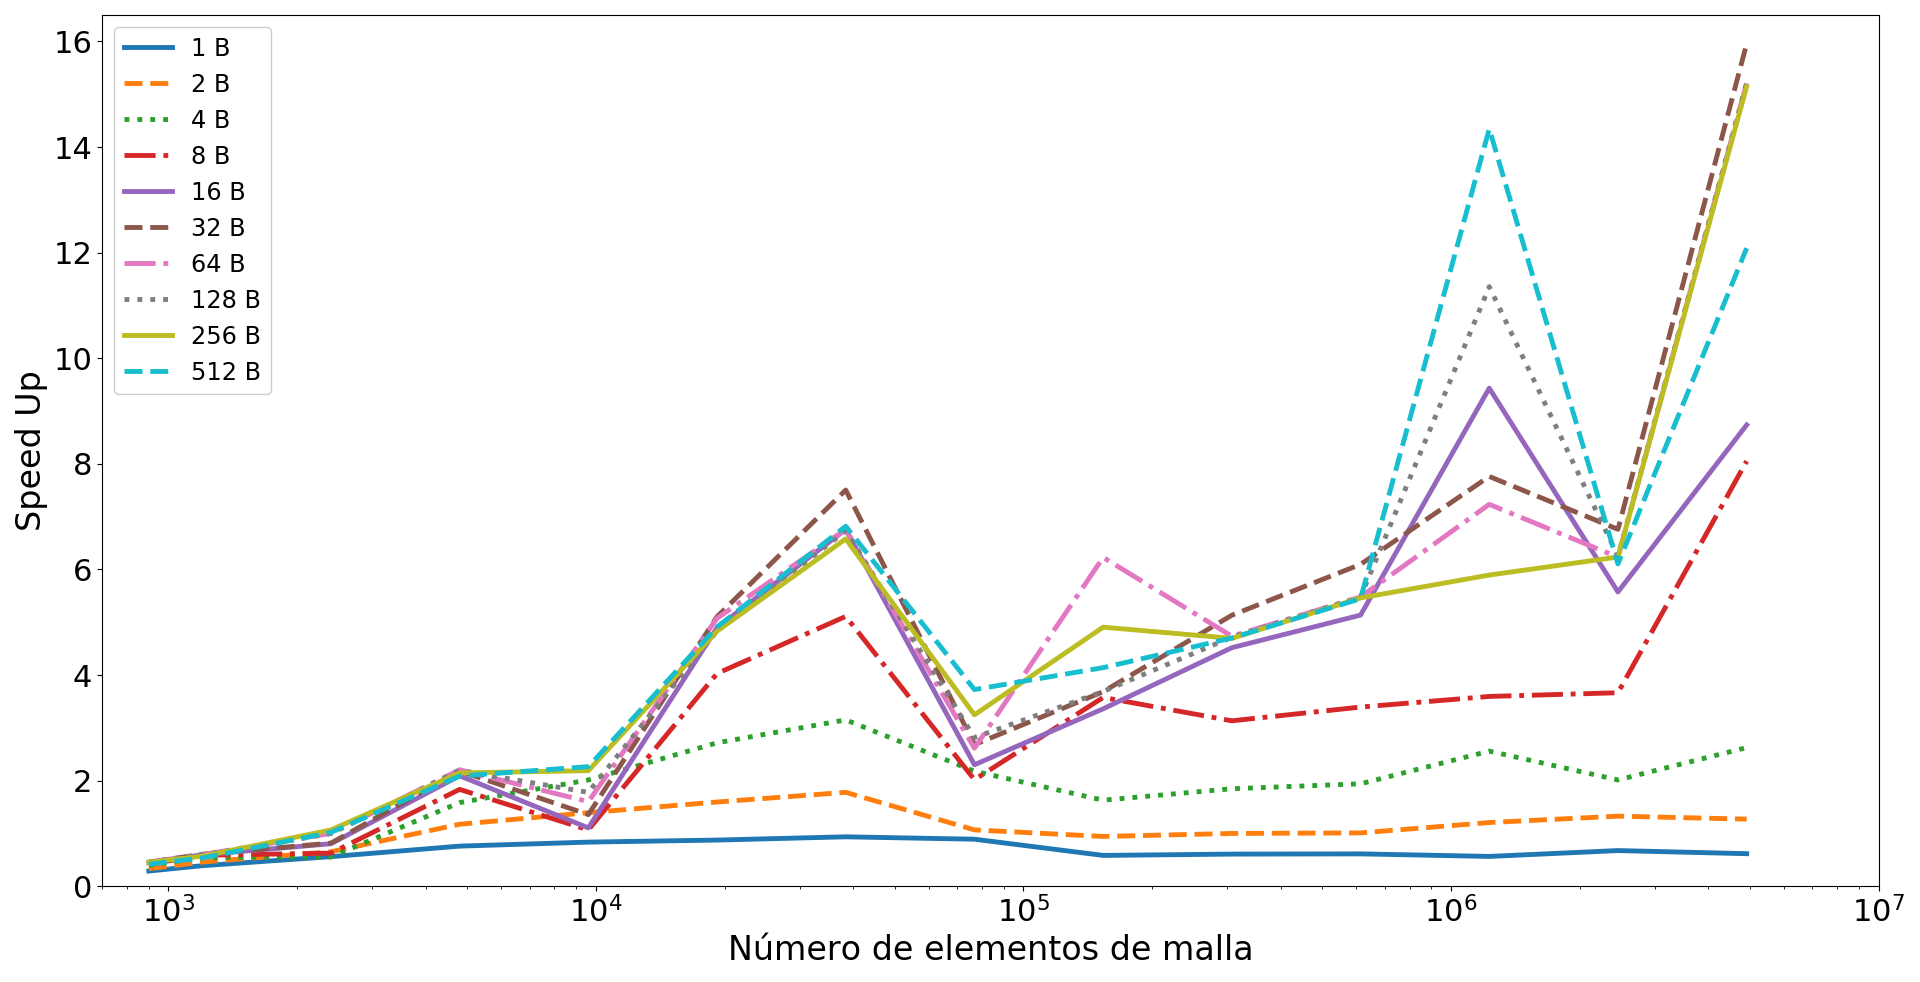
\includegraphics[width=\textwidth]{figs/cap4/s_970_VdW_simple_10}
	\caption{SU realizado para el problema de la Estratificación de un fluido Van dar Waals en simple precisión con una CPU Intel Core i7-4770 y GPU NVIDIA GeForce GTX 970.} 
	\label{fig:s_970_VdW_simple_10}	
\end{figure}

\begin{figure}[h!]
	\centering
	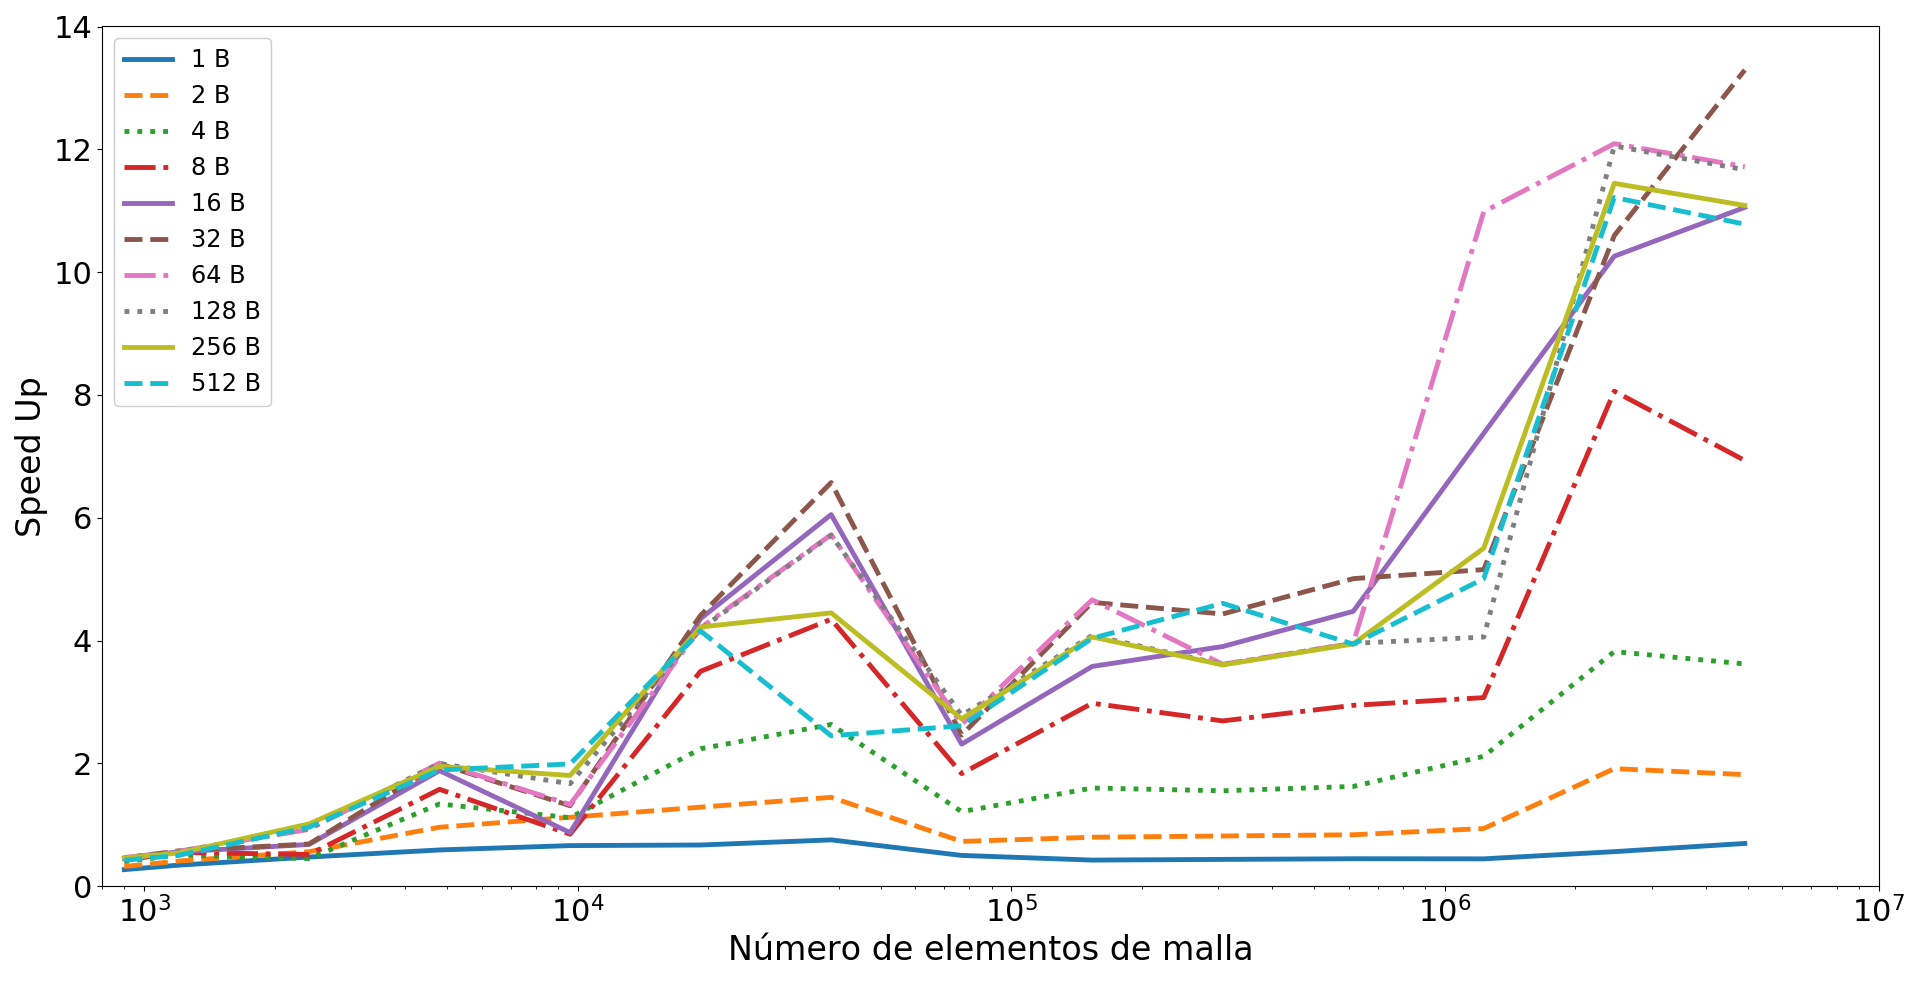
\includegraphics[width=\textwidth]{figs/cap4/s_970_VdW_double_10}
	\caption{SU realizado para el problema de la Estratificación de un fluido Van dar Waals en doble precisión con una CPU Intel Core i7-4770 y GPU NVIDIA GeForce GTX 970.} 
	\label{fig:s_970_VdW_double_10}	
\end{figure}

\newpage

Las Figuras (\ref{fig:s_970_VdW_simple_10}) y (\ref{fig:s_970_VdW_double_10}) muestran el SU obtenido en simple precisión y doble precisión respectivamente. El mejor resultado en ambos casos se obtuvo para un número de \textit{thread block} igual a 32, donde la mejora fue de 15.95 y 13.29 en simple y doble precisión respectivamente, para el mayor número de elementos de malla.

La Figura (\ref{fig:c_970_VdW_cuda_10}) muestra el ${SU}_p$ del código de \textsc{Cuda C} en la GPU NVIDIA GeForce GTX 970. Para un número de \textit{thread block} igual a 32, el tiempo de cálculo en doble precisión es 1,25 veces mayor que en simple precisión en el mayor número de elementos de malla calculado. Se reporta únicamente el resultado para esa cantidad de \textit{thread block}, debido a que los resultados de las Figuras (\ref{fig:s_760_VdW_simple_10}) y (\ref{fig:s_760_VdW_double_10}) indican que es el que tiene un mayor SU.


\begin{figure}[h!]
	\centering
	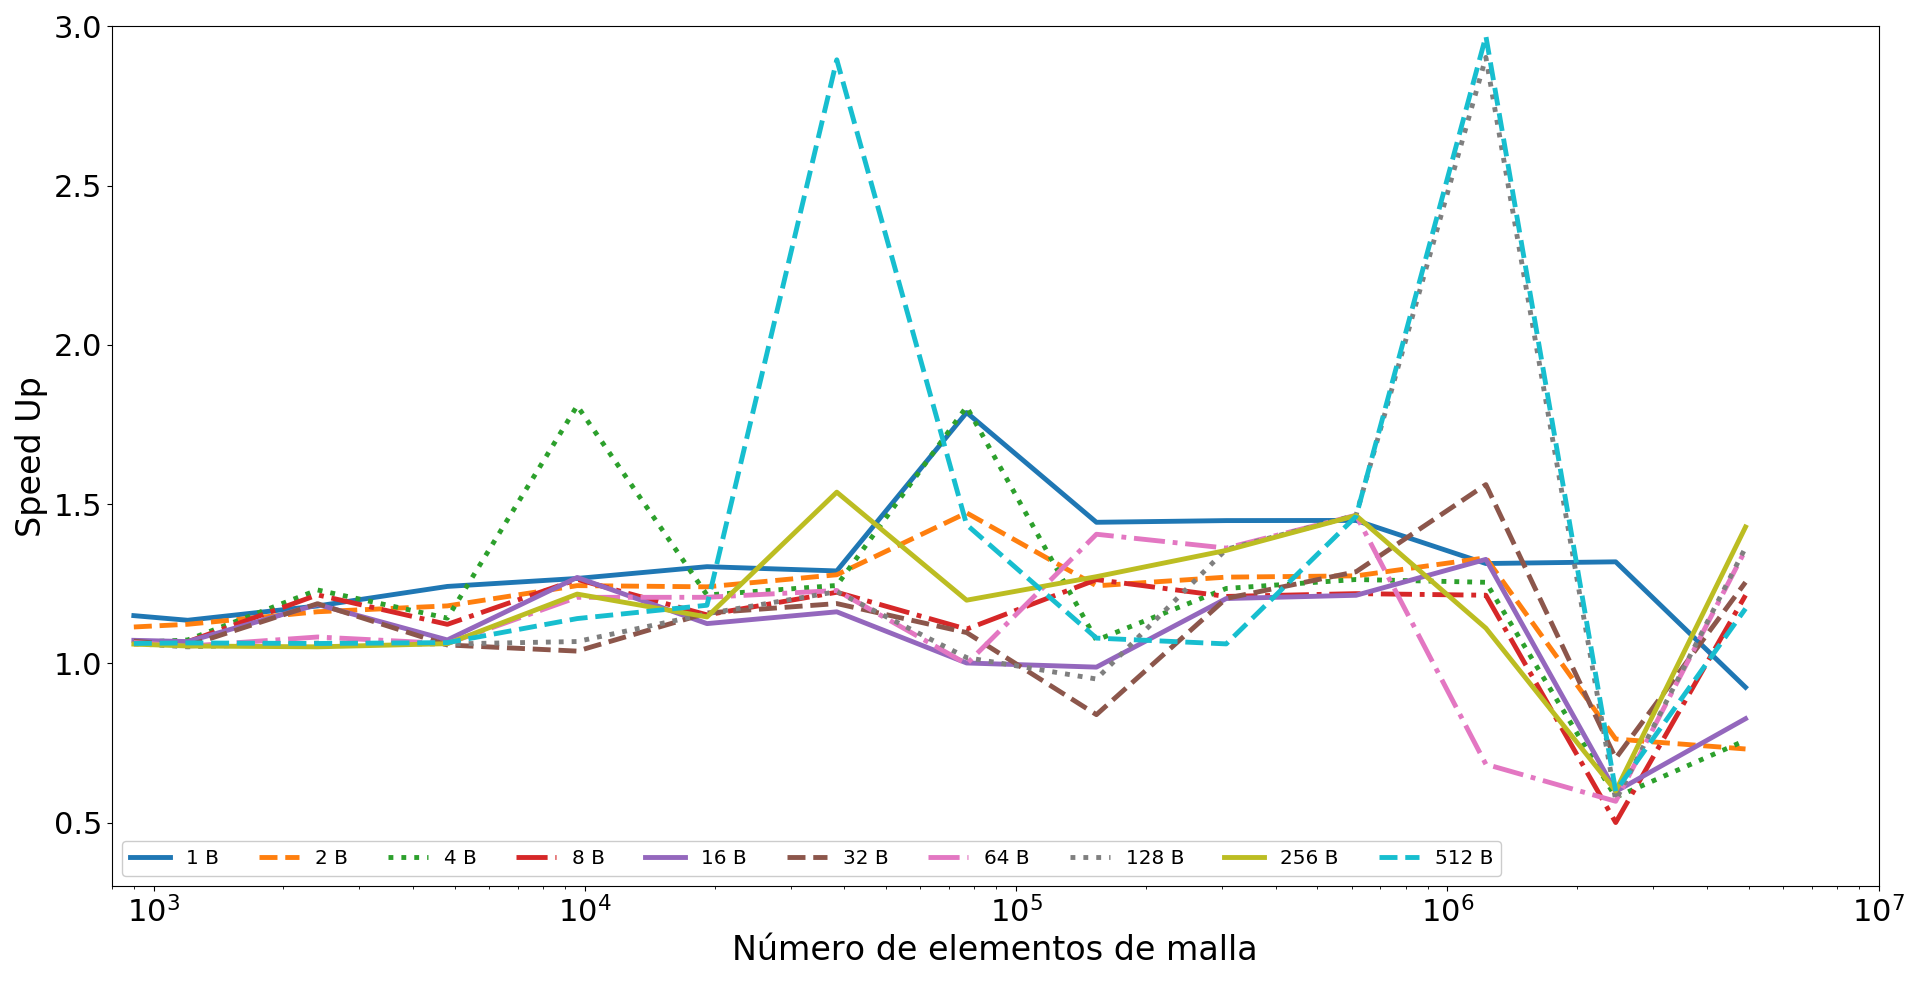
\includegraphics[width=\textwidth]{figs/cap4/c_970_VdW_cuda_10}
	\caption{$SU_p$ realizado para el problema de la Estratificación de un fluido Van der Waals en en el código de \textsc{Cuda C} con la GPU NVIDIA GeForce GTX 970.} 
	\label{fig:c_970_VdW_cuda_10}	
\end{figure}


En este problema las mejoras de implementación del código en \textsc{Cuda C} con respecto a \textsc{C} son considerables, y se puede observar en el índice SU. En el caso de la GPU NVIDIA GeForce GTX 760 se obtuvo un SU de 13,26 y 7,88 para simple y doble precisión respectivamente. Por otro lado en la GPU NVIDIA GeForce GTX 970 se obtuvo un SU de15,95 y 13,29 en simple y doble precisión respectivamente.

Como se mecionó anteriormente, en este problema de estratficación de fluido VdW pudo observarse que la implementación en \textsc{Cuda C} produce una mejora significativa en el tiempo de cálculo con respecto la la implementación equivalente en \textsc{C}. Para este caso, sin embargo, se observó que el SU máximo es inferior al alcanzado en el problema de la Construcción de Maxwell, es decir, con una única LBE.

\newpage
\newpage
\section{Generación de burbujas sobre una superficie horizontal calefaccionada (2D)}

Mediante este problema se busca reproducir la fenomenología asociada a los procesos de transferencia de calor en ebullición, demostrando la potencialidad del método. 

La diferencia del problema de la estratificación de VdW con el de la generación de burbujas, radica en que el primero es unidimensional y el segundo es bidimensional. A su vez, la aplicación del código cambia únicamente en realizar una función que imponga como condición de contorno un área de la superficie calefaccionada.

A partir de las mismas bibliotecas utilizadas anteriormente y cambiando una única función, se obtuvo como resultado el fenómeno de formación, crecimiento y desprendimiento de una burbuja. Para ello se utilizaron los siguientes parámetros de LBM:
{\footnotesize \begin{align*}
diag(\mathbf{\Lambda}) & = 
\begin{bmatrix}
1.0 & 1.25 & 1.0 & 1.0 & 1.1 & 1.0 & 1.1 & 1.3 & 1.3 \\
\end{bmatrix}\\
diag(\mathbf{Q}) & = 
\begin{bmatrix}
1.0 & 1.0 & 1.0 & 1.55 & 1.0 & 1.55 & 1.0 & 1.0 & 1.0 \\
\end{bmatrix}\\
\alpha_{1} & = -2.0 \qquad 	\alpha_{2} = 2.0 \qquad C_{v} = 5.0\\
G & = -1.0 \quad c = 1.0 \quad \sigma = 0.125 \quad a = 1.0 \quad b = 4.0 \\
\mathbf{g} & = (0.0 \quad -8.0^{-6} \quad 0.0 ) \qquad \rho_c = \frac{1}{12} \qquad T_c = 0.074074074
\end{align*}}
El tamaño de grilla utilizado fue de L = 300 y H = 500 basándose en el esquema del panel izquierdo de la Figura (\ref{fig:esquema_VdW}), donde la superficie calefaccionada se encuentra en el centro del lado L y posee un tamaño de 12 elementos de malla. La temperatura de calefacción $T_{heat} = T_c$  y el resto de la superficie se encuentra a $T = 0.8 T_c$ con la parte superior de la cavidad está a $T = 0.99 T_c$. La separación inicial de las dos fases se encuentra en $y = 350$, donde $\rho = 0.1610588 \> si \> y \in [0,350]$ y $\rho = 0.0199722$ $y$ para $(350,500]$.

El resultado que se obtuvo para 5000, 10000, 20000, 25000, 30000, 35000, 40000, 45000 y 50000 pasos de tiempo se encuentra en la Figura (\ref{fig:burbujas_760_doble_cuda}), realizada en la GPU NVIDIA GeForce GTX 760 para doble precisión. Adicionalmente en la Figura (\ref{fig:bb_simple_doble_760}) se encuentra para 25000 pasos de tiempo la comparación entre simple y doble precisión realizado en la GPU NVIDIA GeForce GTX 760. También se realizó la comparación entre el resultado obtenido para 45000 pasos de tiempo entre la CPU Intel Core i7-3770 y la GPU NVIDIA GeForce GTX 760 en simple precisión  en la Figura (\ref{fig:bb_CPU_GPU_simple}). Al analizar los resultados de la CPU y GPU con sus precisiones, y comparándolas entre todos los casos realizados, resultan similares en primera instancia.

Con ésto se demuestra que la reproducción de un fenómeno complejo como la ebullición, puede ser resuelta mediante un LBM de sencilla aplicación y a su vez con un costo computacional bajo, comparando con métodos de elementos finitos o diferencias finitas \cite{guo2013lattice}.

%Si se observan las Figuras (\ref{fig:burbujas_760_simple}) y (\ref{fig:burbujas_760_doble}), que fueron realizadas por medio de la CPU Intel Core i7-3770 a simple vista no se halla ninguna diferencia entre los resultados en distintas precisiones. Por otro lado para las figuras las Figuras (\ref{fig:burbujas_760_simple_cuda}) y (\ref{fig:burbujas_760_doble_cuda}) sucede exactamente lo mismo en cuanto a las precisiones.
%Por lo tanto no se halla ninguna diferencia en primera instancia en utilizar las GPU en lugar de la CPU en cuanto al resultado esperado, como así también, tampoco se encontró una diferencia notable en cuanto a utilizar distintas precesiones. 



\iffalse

\begin{figure}[H]
	\centering
	\begin{subfigure}{0.25\textwidth}
		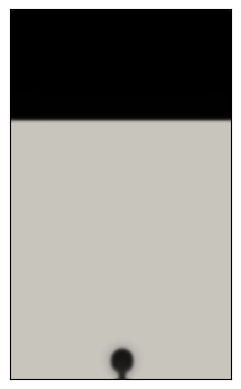
\includegraphics[width=\linewidth]{figs/cap4/bb_760_s5}
		\caption{t = 5000}
		\label{fig:1}
	\end{subfigure}\hfil 
	\begin{subfigure}{0.25\textwidth}
		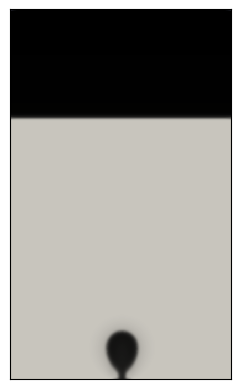
\includegraphics[width=\linewidth]{figs/cap4/bb_760_s10}
		\caption{t = 10000}
		\label{fig:2}
	\end{subfigure}\hfil 
	\begin{subfigure}{0.25\textwidth}
		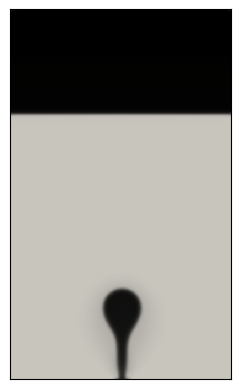
\includegraphics[width=\linewidth]{figs/cap4/bb_760_s20}
		\caption{t = 20000}
		\label{fig:3}
	\end{subfigure}
	
	\medskip
	\begin{subfigure}{0.25\textwidth}
		
\includegraphics[width=\linewidth]{figs/cap4/bb_760_s25}
		\caption{t = 25000}
		\label{fig:4}
	\end{subfigure}\hfil  
	\begin{subfigure}{0.25\textwidth}
		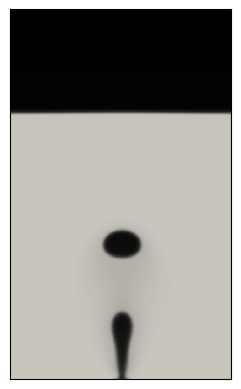
\includegraphics[width=\linewidth]{figs/cap4/bb_760_s30}
		\caption{t = 30000}
		\label{fig:5}
	\end{subfigure}\hfil 
	\begin{subfigure}{0.25\textwidth}
		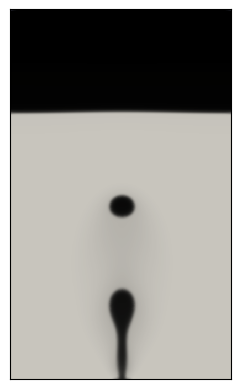
\includegraphics[width=\linewidth]{figs/cap4/bb_760_s35}
		\caption{t = 35000}
		\label{fig:6}
	\end{subfigure}
	
	\medskip
	\begin{subfigure}{0.25\textwidth}
		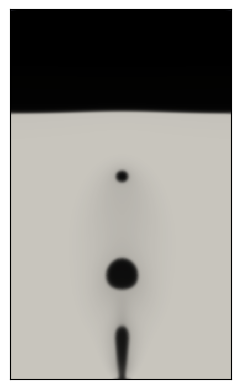
\includegraphics[width=\linewidth]{figs/cap4/bb_760_s40}
		\caption{t = 40000}
		\label{fig:7}
	\end{subfigure}\hfil
	\begin{subfigure}{0.25\textwidth}
		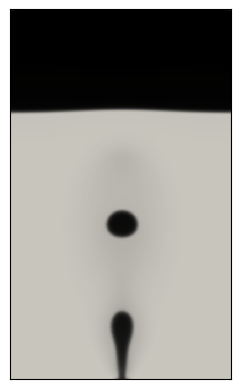
\includegraphics[width=\linewidth]{figs/cap4/bb_760_s45}
		\caption{t = 45000}
		\label{fig:8}
	\end{subfigure}\hfil 
	\begin{subfigure}{0.25\textwidth}
		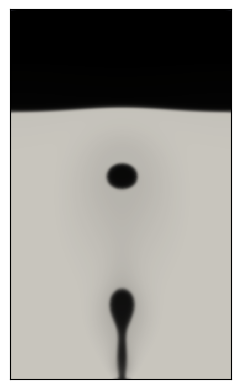
\includegraphics[width=\linewidth]{figs/cap4/bb_760_s50}
		\caption{t = 50000}
		\label{fig:9}
	\end{subfigure}
	\caption{Creación y desarrollo de una burbuja a partir de una superficie horizontal calefaccionada. Realizado por medio de la CPU Intel Core i7-3770 en simple precisión. }
	\label{fig:burbujas_760_simple}
\end{figure}

\newpage

\newpage

\begin{figure}[H]
	\centering
	\begin{subfigure}{0.25\textwidth}
		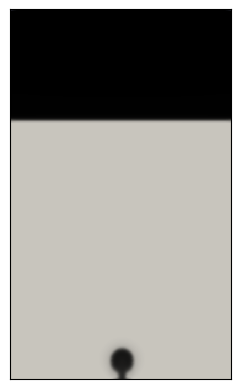
\includegraphics[width=\linewidth]{figs/cap4/bb_760_d5}
		\caption{t = 5000}
		\label{fig:1}
	\end{subfigure}\hfil 
	\begin{subfigure}{0.25\textwidth}
		
\includegraphics[width=\linewidth]{figs/cap4/bb_760_d10}
		\caption{t = 10000}
		\label{fig:2}
	\end{subfigure}\hfil 
	\begin{subfigure}{0.25\textwidth}
		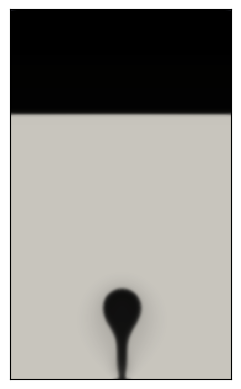
\includegraphics[width=\linewidth]{figs/cap4/bb_760_d20}
		\caption{t = 20000}
		\label{fig:3}
	\end{subfigure}
	
	\medskip
	\begin{subfigure}{0.25\textwidth}
		
\includegraphics[width=\linewidth]{figs/cap4/bb_760_d25}
		\caption{t = 25000}
		\label{fig:4}
	\end{subfigure}\hfil  
	\begin{subfigure}{0.25\textwidth}
		
\includegraphics[width=\linewidth]{figs/cap4/bb_760_d30}
		\caption{t = 30000}
		\label{fig:5}
	\end{subfigure}\hfil 
	\begin{subfigure}{0.25\textwidth}
		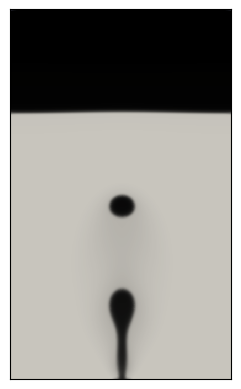
\includegraphics[width=\linewidth]{figs/cap4/bb_760_d35}
		\caption{t = 35000}
		\label{fig:6}
	\end{subfigure}
	
	\medskip
	\begin{subfigure}{0.25\textwidth}
		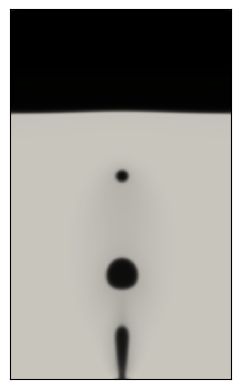
\includegraphics[width=\linewidth]{figs/cap4/bb_760_d40}
		\caption{t = 40000}
		\label{fig:7}
	\end{subfigure}\hfil
	\begin{subfigure}{0.25\textwidth}
		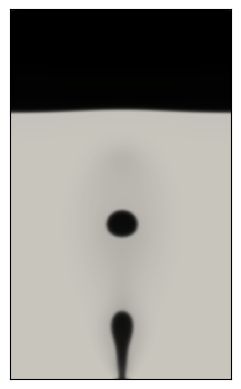
\includegraphics[width=\linewidth]{figs/cap4/bb_760_d45}
		\caption{t = 45000}
		\label{fig:8}
	\end{subfigure}\hfil 
	\begin{subfigure}{0.25\textwidth}
		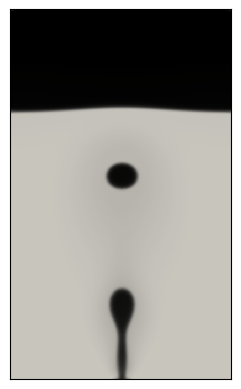
\includegraphics[width=\linewidth]{figs/cap4/bb_760_d50}
		\caption{t = 50000}
		\label{fig:9}
	\end{subfigure}
	\caption{Creación y desarrollo de una burbuja a partir de una superficie horizontal calefaccionada. Realizado por medio de la CPU Intel Core i7-3770 en doble precisión.}
	\label{fig:burbujas_760_doble}
\end{figure}

\newpage

\newpage

\begin{figure}[H]
	\centering
	\begin{subfigure}{0.25\textwidth}
		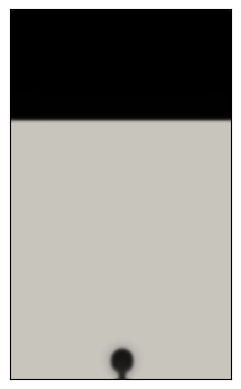
\includegraphics[width=\linewidth]{figs/cap4/cuda_bb_760_s5}
		\caption{t = 5000}
		\label{fig:1}
	\end{subfigure}\hfil 
	\begin{subfigure}{0.25\textwidth}
		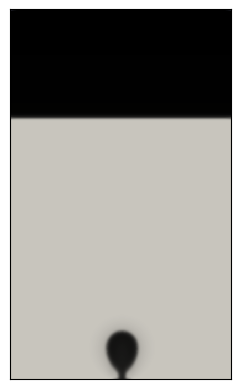
\includegraphics[width=\linewidth]{figs/cap4/cuda_bb_760_s10}
		\caption{t = 10000}
		\label{fig:2}
	\end{subfigure}\hfil 
	\begin{subfigure}{0.25\textwidth}
		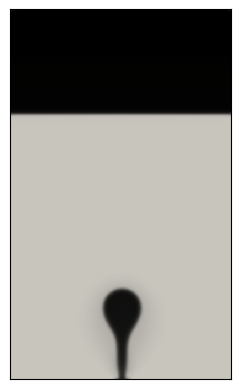
\includegraphics[width=\linewidth]{figs/cap4/cuda_bb_760_s20}
		\caption{t = 20000}
		\label{fig:3}
	\end{subfigure}
	
	\medskip
	\begin{subfigure}{0.25\textwidth}
		
\includegraphics[width=\linewidth]{figs/cap4/cuda_bb_760_s25}
		\caption{t = 25000}
		\label{fig:4}
	\end{subfigure}\hfil  
	\begin{subfigure}{0.25\textwidth}
		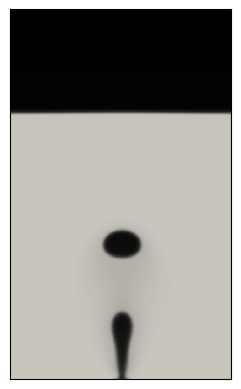
\includegraphics[width=\linewidth]{figs/cap4/cuda_bb_760_s30}
		\caption{t = 30000}
		\label{fig:5}
	\end{subfigure}\hfil 
	\begin{subfigure}{0.25\textwidth}
		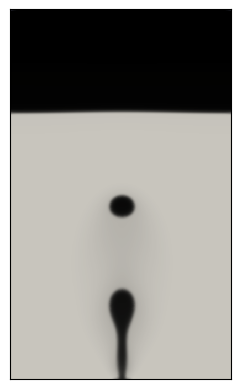
\includegraphics[width=\linewidth]{figs/cap4/cuda_bb_760_s35}
		\caption{t = 35000}
		\label{fig:6}
	\end{subfigure}
	
	\medskip
	\begin{subfigure}{0.25\textwidth}
		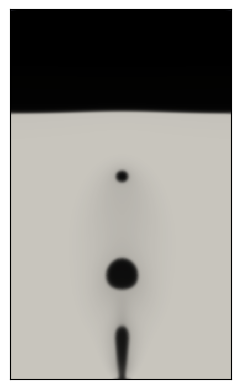
\includegraphics[width=\linewidth]{figs/cap4/cuda_bb_760_s40}
		\caption{t = 40000}
		\label{fig:7}
	\end{subfigure}\hfil
	\begin{subfigure}{0.25\textwidth}
		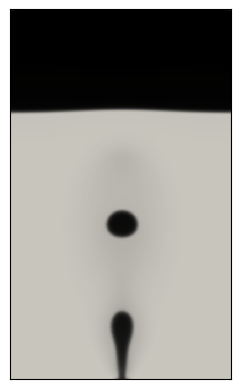
\includegraphics[width=\linewidth]{figs/cap4/cuda_bb_760_s45}
		\caption{t = 45000}
		\label{fig:8}
	\end{subfigure}\hfil 
	\begin{subfigure}{0.25\textwidth}
		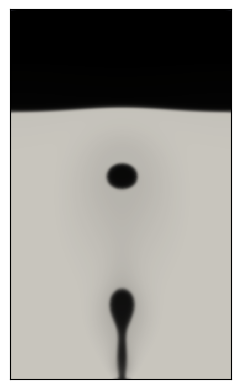
\includegraphics[width=\linewidth]{figs/cap4/cuda_bb_760_s50}
		\caption{t = 50000}
		\label{fig:9}
	\end{subfigure}
	\caption{Creación y desarrollo de una burbuja a partir de una superficie horizontal calefaccionada. Realizado por medio de la GPU NVIDIA GeForce GTX 760 en simple precisión. }
	\label{fig:burbujas_760_simple_cuda}
\end{figure}

\newpage

\fi

\newpage

\begin{figure}[H]
	\centering
	\begin{subfigure}{0.25\textwidth}
		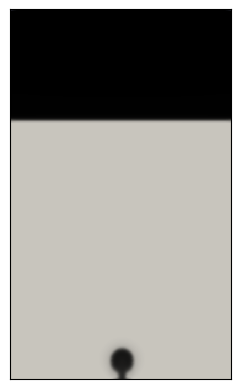
\includegraphics[width=\linewidth]{figs/cap4/cuda_bb_760_d5}
		\caption{t = 5000}
		\label{fig:1}
	\end{subfigure}\hfil 
	\begin{subfigure}{0.25\textwidth}
		
\includegraphics[width=\linewidth]{figs/cap4/cuda_bb_760_d10}
		\caption{t = 10000}
		\label{fig:2}
	\end{subfigure}\hfil 
	\begin{subfigure}{0.25\textwidth}
		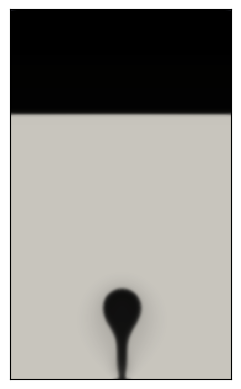
\includegraphics[width=\linewidth]{figs/cap4/cuda_bb_760_d20}
		\caption{t = 20000}
		\label{fig:3}
	\end{subfigure}
	
	\medskip
	\begin{subfigure}{0.25\textwidth}
		
\includegraphics[width=\linewidth]{figs/cap4/cuda_bb_760_d25}
		\caption{t = 25000}
		\label{fig:4}
	\end{subfigure}\hfil  
	\begin{subfigure}{0.25\textwidth}
		\includegraphics[width=\linewidth]{figs/cap4/cuda_bb_760_d30}
		\caption{t = 30000}
		\label{fig:5}
	\end{subfigure}\hfil 
	\begin{subfigure}{0.25\textwidth}
		\includegraphics[width=\linewidth]{figs/cap4/cuda_bb_760_d35}
		\caption{t = 35000}
		\label{fig:6}
	\end{subfigure}
	
	\medskip
	\begin{subfigure}{0.25\textwidth}
		\includegraphics[width=\linewidth]{figs/cap4/cuda_bb_760_d40}
		\caption{t = 40000}
		\label{fig:7}
	\end{subfigure}\hfil
	\begin{subfigure}{0.25\textwidth}
		\includegraphics[width=\linewidth]{figs/cap4/cuda_bb_760_d45}
		\caption{t = 45000}
		\label{fig:8}
	\end{subfigure}\hfil 
	\begin{subfigure}{0.25\textwidth}
		\includegraphics[width=\linewidth]{figs/cap4/cuda_bb_760_d50}
		\caption{t = 50000}
		\label{fig:9}
	\end{subfigure}
	\caption{Creación y desarrollo de una burbuja a partir de una superficie horizontal calefaccionada. Realizado por medio de la GPU NVIDIA GeForce GTX 760 en doble precisión.}
	\label{fig:burbujas_760_doble_cuda}
\end{figure}

\newpage

\begin{figure}[H]
\centering
	\begin{subfigure}{0.35\textwidth}
		\includegraphics[width=\linewidth]{figs/cap4/cuda_bb_760_s25}
		\caption{Simple precisión}
		\label{fig:bb_sp_760}\hfil
	\end{subfigure}
	\begin{subfigure}{0.35\textwidth}
	\includegraphics[width=\linewidth]{figs/cap4/cuda_bb_760_d25}
	\caption{Doble precisión}
	\label{fig:bb_dp_760}\hfil
	\end{subfigure}

\caption{Creación y desarrollo de una burbuja para 25000 pasos de tiempo realizado en la GPU NVIDIA GeForce GTX 760. Izquierda: Simple precisión. Derecha: Doble precesión.}
\label{fig:bb_simple_doble_760}
\end{figure}

\begin{figure}[H]
	\centering
	\begin{subfigure}{0.35\textwidth}
		\includegraphics[width=\linewidth]{figs/cap4/bb_760_s45}
		\caption{Intel Core i7 - 3770}
		\label{fig:b_sp_760}\hfil
	\end{subfigure}
	\begin{subfigure}{0.35\textwidth}
		\includegraphics[width=\linewidth]{figs/cap4/cuda_bb_760_s45}
		\caption{NVIDIA GeForce GTX 760}
		\label{fig:b_dp_760}\hfil
	\end{subfigure}
	
	\caption{Creación y desarrollo de una burbuja para 45000 pasos de tiempo en simple precisión. Izquierda: Realizado por medio de la CPU Intel Core i7-3770. Derecha: Realizado por medio de la GPU NVIDIA GeForce GTX 760.}
	\label{fig:bb_CPU_GPU_simple}
\end{figure}
\newpage

\section{Uso de \textsc{PyCuda}}

La realización de los códigos numéricos mediante \textsc{C} y \textsc{Cuda C} tenían como primera finalidad conocer cuál es la ganancia en tiempo de cálculo realizando la implementación en GPU, por otro lado desarrollar código en \textsc{Cuda C}, para luego compilarlo en formato \textsc{ptx} y ser utilizado en \textsc{Python} por medio del módulo \textsc{PyCuda} del mismo.

Debido a la falta de tiempo en el desarrollo del Proyecto Integrador no se pudo completar el desarrollo de módulos de \textsc{Python} que implementen con \textsc{PyCuda} los \textit{kernels} compilados previemente, con el objetivo de resolver los problemas de construcción de Maxwell, estratificación de fluido VdW y generación de burbujas sobre una placa calefaccionada.  Sin embargo, pudo analizarse el uso de \textit{kernels} individuales, como el que realiza el cálculo de la densidad macroscópica (Ec.(\ref{eq:rho_py})) en todos los nodos de la grilla.

\begin{equation}
\rho = \sum_{\alpha} f_{\alpha}
\label{eq:rho_py}
\end{equation}

Para éste análisis se inicializó a $f$ con valores aleatorios, haciendo una repetición de la ejecución de la función 100000 veces para realizar la toma de tiempo. Se varió el tamaño de la grilla, de manera que ésta siempre fuese cuadrada, respetando un número de nodos de potencia de 2 en los lados del cuadrado. La cantidad de \textit{thread blocks} que se utilizó para realizar la comparación en el código fue de potencia de 2. El tamaño de la grilla varió de 16x16 hasta 4096x4906 y la cantidad de \textit{thread blocks} utilizado es de 1 a 512.

Al  realizar la implementación de un \textit{kernel} de \textsc{Cuda C} en \textsc{Python}, se espera que el tiempo de cálculo en \textsc{Python} sea más lento que en \textsc{Cuda C}, debido a que el primer lenguaje es interpretado. Debido a lo mencionado es que se define el índice \textit{Speed Down} (SD), donde \textit{t} es el tiempo de cálculo. SD es una medida de cuánto es la demora de un código respecto a otro y se calcula de la siguiente forma :

\begin{align}
SD = \frac{t_{\>PyCuda}}{t_{\>Cuda \> C}} 
\end{align} 


\title{\textbf{NVIDIA GeForce GTX 760}}
\newline

La Figura (\ref{fig:s_cuda_760_test_simple_10}) muestra el SU para la GPU NVIDIA GeForce GTX 760, donde se observa que la mayor ganancia obtenida es de 3,2 para 64 \textit{thread blocks}. Por otro lado, en la Figura (\ref{fig:s_py_760_test_simple_10}) se muestra el SD, en donde puede verse que el menor valor alcanzado es de 1,14 para 128 y 512  \textit{thread blocks}.

\begin{figure}[h!]
	\centering
	\includegraphics[width=\textwidth]{figs/cap4/s_cuda_760_test_simple_10}
	\caption{SU entre \textsc{C} y \textsc{Cuda C} para la función de obtención de la densidad con la GPU NVIDIA GeForce GTX 760 en simple precisión.} 
	\label{fig:s_cuda_760_test_simple_10}	
\end{figure}



%\begin{figure}[h!]
%	\centering
%	\includegraphics[width=\textwidth]{figs/cap4/s_py_c_760_test_simple_10}
%	\caption{Speed Up realizado entre PyCUDA y C para la función de obtensión de la densidad con la GPU NVIDIA GeForce GTX 760 en simple precisión.} 
%	\label{fig:s_py_c_760_test_simple_10}	
%\end{figure}


\begin{figure}[h!]
	\centering
	\includegraphics[width=\textwidth]{figs/cap4/s_py_760_test_simple_10}
	\caption{SD realizado entre \textsc{PyCuda} y \textsc{Cuda} para la función de obtención de la densidad con la GPU NVIDIA GeForce GTX 760 en simple precisión.} 
	\label{fig:s_py_760_test_simple_10}	
\end{figure}


\newpage
%
\title{\textbf{NVIDIA GeForce GTX 970}}\\

La Figura (\ref{fig:s_cuda_970_test_simple_10}) muestra el SU para la GPU NVIDIA GeForce GTX 970, donde se observa que la mayor ganancia obtenida es de 4,8 para 64 \textit{thread blocks}. Por otro lado, en la Figura (\ref{fig:s_py_970_test_simple_10}) se muestra el SD, en donde puede verse que los menores valores alcanzados son 1,08 y 1,10 para 128 y 512  \textit{thread blocks} respectivamente.


\begin{figure}[h!]
	\centering
	\includegraphics[width=\textwidth]{figs/cap4/s_cuda_970_test_simple_10}
	\caption{SU realizado entre \textsc{C} y \textsc{Cuda C} para la función de obtención de la densidad con la GPU NVIDIA GeForce GTX 970 en simple precisión.} 
	\label{fig:s_cuda_970_test_simple_10}	
\end{figure}

\begin{figure}[h!]
	\centering
	\includegraphics[width=\textwidth]{figs/cap4/s_py_970_test_simple_10}
	\caption{SD para la función de obtención de la densidad con la GPU NVIDIA GeForce GTX 970 en simple precisión.} 
	\label{fig:s_py_970_test_simple_10}	
\end{figure}

%\section{Análisis}

\newpage
Luego de haber realizado la implementación de un \textit{kernel} de \textsc{Cuda C} en un \textit{script} de \textsc{Python} por medio del módulo \textsc{PyCuda}, se observa que el tiempo de cálculo se incrementa. La variación del incremento, que se mide por el índice SD depende en gran medida de la cantidad de \textit{thread blocks} utilizados, al igual que el tamaño de la grilla.

Debido a que se pretende utilizar con la mayor eficiencia posible los \textit{kernels} en \textit{Python}, debe ejecutarse con la cantidad de \textit{thread blocks} que minimicen SD. De las pruebas realizadasse obtuvo que para la GPU NVIDIA GeForce GTX 760 con 128 y 512  \textit{thread blocks} el valor de SD se encuentra cercano al 15 \% , mientras que en la GPU NVIDIA GeForce GTX 970 ese valor esta cercano al 10 \%.

Es de importancia el desarrollo de códigos numéricos para que sean eficientes en el tiempo de cálculo, y que el desarrollo del mismo no implique un gran insumo de tiempo. Por lo último mencionado realizar códigos en \textsc{Python} es eficiente al ser un lenguaje interpretado y no tener que reservar memoria, liberar memoria o declarar variables entre otros. Los módulos de \textsc{Python} tienen sus bibliotecas realizadas mayormente en \textsc{C} y \textsc{Cuda C} para que sean eficientes y debido a ello es conveniente la utilización de sus módulos, que ya poseen las funciones que se necesita, además siendo eficientes. 

De esta forma, se observó que resulta posible continuar con la extensión y generalización de herramientas de cálculo eficientes utilizando una combinación adecuada de los lenguajes mencionados.


% por medio de alguno de sus módulos utiliar la función creada. , debido a que no se incrementa mucho el tiempo de cálculo al utiliar \textit{kernels} previamente compilados. 



% Al momento de realizar una función específica se puede recurrir a módulos de \textsc{Python} que probablemente tengan ya implementado lo que se pretende hacer. Entonces se puede utilizar \textit{Python} para progresar rápido en porcentualmente en la terminación un proyecto, en donde la optimización del mismo puede ser llevada a cabo mediante módulos de \textit{Python}. casi el tiempo de cálculo que se rlo utilizando el módulo de \textit{PyCuda}
%
% al hecho concreto de programar. Por ello es que se recomienda que sean 
%
%
%
%Para realizar un balance de la conveniencia del uso de \textsc{Python} se deben tener en cuenta viarios factores, el siguiente análisis sólo toma tres (3).
%
%
%El primero es la facilidad de programar en paralelo mediante \textsc{Cuda C} debido a su extensión de \textsc{C}. Lo segundo es la facilidad y fluidez de programación en \textit{Python} mediante el uso de clases,  objetos y los módulos disponibles que posee. Lo tercero es la implementación de los \textit{kernels} mediante el módulo \textsc{PyCuda}.
%
%Para el desarrollo de proyectos complejos, como el presente caso, se consume mucho tiempo tener que realizarrealizar 
%Debido a que el desarrollo de LBM para casos más complejos y genéricos resulta un insumo importante de tiempo, 
%
%Al realizar un balance de la facilidad de realizar código en \textsc{Python} por ser un lenguaje interpretado
%Por lo que no se pierde mucha eficiencia programando en el lenguaje de \textsc{Python}.

\newpage
%\section{Optimización}
%
%Con lo realizado hasta el momento se logró una implementación válida de LBM en los lenguajes de programación \textit{C} y \textit{Cuda C}, en donde se obtuvo un SU de hasta 19 y 23 en las GPU NVIDIA GeForce GTX 760 y GPU NVIDIA GeForce GTX 970 respectivamente para el problema de la construcción de Maxwell en simple precisión.
%
%Para obtener un mejor resultado posible se debe aprovechar la arquitectura de hardware de la GPU es necesario utilizar nuevas técnicas de las que ya se conocen para las CPU, es por eso que se decidió realizar el cambio de todas las funciones \textcolor{blue}{for} por las funciones \textcolor{blue}{while}. Éste cambio se encuentra argumentado, debido a que la estructura de la memoria utilizada en la GPU es un \textit{array} y que en las GPU no se permite una reserva de memoria de un puntero en el \textit{device memory} como se realizaba típicamente en una CPU. El cambio también fue realizado al tener todos los copmponentes del \textit{array} ocupados, ya que la condición lógica del \textcolor{blue}{while} es más provechosa que la de \textcolor{blue}{for} en éste tipo de situaciones.
%
%Se pude implementar la optimización para la PC que contaba con una CPU Intel Core i7-4770 y GPU NVIDIA GeForce GTX 970, en el problema de la construcción de Maxwell para simple precisión. El SU máximo alcanzado es de 33,22 llevado a cabo con 32 \textit{thread block} y los valores obtenidos se pueden ver a continuación:
%
%\begin{figure}[h!]
%	\centering
%	\includegraphics[width=0.99\textwidth]{figs/cap4/version_2_970_MxC_cuda}
%	\caption{SU realizado para el problema de la Construcción de Maxwell en simple precisión con una CPU Intel Core i7-4770 y GPU NVIDIA GeForce GTX 970 con la optimización implementada.} 
%	\label{fig:s_970_MxC_simple_20}	
%\end{figure}
%
%La implementación realizada como optimización produjo un aumento de 42 \% con respecto a la versión anterior del código.

%%% Local Variables: 
%%% mode: latex
%%% TeX-master: "template"
%%% End: 
